\section{Preface}
\textit{The following chapter contains work from the paper \textbf{Detailed analysis of the double functional maps
in EphA3 knock-in mice} researched and written in collaboration with David Willshaw at the University of Edinburgh \cite{Willshaw2022-fs}. The research aim was to rigorously investigate the claim that the EphA3 heterozygote is on the border of a bifurcation point where it can phenotypically present itself in a stochastic manner as a wild-type, homozygote, or some mixed state in between, dependent on the neural activity patterns \cite{Owens2015-zv}. The biological data analysis using the lattice method was performed by primarily by David Willshaw and will be included in this chapter in Section \ref{section:davidsresults} to contextualise my theoretical results presented thereafter. The predominate focus of the chapter will be to recreate the experimental pipeline computationally and use modelling efforts to interrogate the central claim of stochasticity in the development of heterozygous mice. } 
\section{Introduction}
The individual effects of chemotaxis and neural activity have been discussed in both experimental and modelling contexts and subsequent theory has been developed for the individual contribution of these mechanisms: chemotaxis establishes a coarse topography on the basis of relative signalling while neural activity works to refine this interaction through a spatio-temporal patterning of spontaneous activity before eye-opening; see Section \ref{section:developmentaltheory} for a complete review and Chapter \ref{chapter:neuralstdp} for a detailed account of modelling activity in the wild-type and $\beta2^{-/-}$ genotype cases. The relative effects that these two developmental systems have on each other is less clearly understood with suggestions that activity patterns may regulate Eph/ephrin expression \cite{Lyngholm2019-fs, Nicol2007-rt}. A recent hypothesis is that chemotaxis and neural activity are finely balanced in the wild-type mouse but stochastic map generation can be achieved by manipulating chemical gradients and thus these mechanisms are ultimately stochastic in nature \cite{Owens2015-zv}. 

This hypothesis was developed by performing intrinsic optical imaging scans on the superior colliculus of several wild-type and mouse mutants: EphA3$^{+/-}$, and EphA3$^{+/+}$ knock-ins and combined EphA3$^{+/-}$$\beta2^{-/-}$. As discussed in Section \ref{sec:epha3} the EphA3 receptor is not endogenous to mouse and it is knocked in on the Islet2 expressing cells in the retina resulting in a boost of EphA receptor in a random salt-and-pepper distribution across the retina \cite{Brown2000-da, Reber2004-wq}. Retrograde DiI injections revealed that in the homozygous knock-in a complete duplicated map is formed: for every retinal injection site there are two termination sites in the superior colliculus along the rostrocaudal axis; see Figures \ref{fig:epha3anatomical} and \ref{fig:epha3collapse}. The heterozygotes follow a similar relationship but the duplicated projections are restricted to the caudal region of the colliculus collapsing into a single projection rostrally \cite{Brown2000-da}. These make it an excellent candidate to study perturbative effects in chemical signalling.

An intrinsic optical imaging scan is performed by stimulating a mouses visual field with a regular periodic signal and measuring the phase of the induced activity in the colliculus: the phase should correlate with the average retinal position of the signal along the stimulating axis; see Section \ref{sec:optical}. Optical imaging scans revealed that the homozygous knock-ins reliably produced a functional double map suggesting that the wild-type and EphA3$^{+/+}$ populations are segregated \cite{Cang2008-ez}. The technique was then performed on heterozygous knock-ins by Owens et. al. (2015) and revealed a highly variable phenotype: it would phenotypically present as a wild-type, a homozygote, and a class of mixed state in between; see Figure \ref{fig:owens}. To understand this variability in the context of activity they disrupted activity patterns by creating a EphA3$^{+/-}\beta2^{-/-}$ mutant and remarkably optical imaging experiments revealed that the variable heterozygous states collapsed into a wild-type phenotype. These results were corroborated with a computational model: the restricted competition Tsigankov-Koulakov model of unified mechanism \cite{Tsigankov2006-uy}. They showed this model can phenomenologically reproduce the EphA3$^{+/+}$ phenotype by adding additional EphA, here called $\Delta R$, in a subset of cells in the retina distributed in a salt-and-pepper fashions. They demonstrated that when this $\Delta R$ was tuned to a point in-between wild-type and homozygous levels the model qualitatively produced maps similar to those observed experimentally. These data were collectively interpreted by Owens et. al. (2015) in the following manner: there exists a fine balance between neural activity and chemotactic developmental mechanisms. The heterozygous knock-in exists on the border of a bifurcation point between the regular wild-type and homozygous mapping. At this bifurcation point the model suggests activity dependent mechanisms stochasticly cause the heterozygote present in a heterogeneous plethora of states. Investigation of this hypothesis of stochastic interaction between developmental mechanisms will be the primary focus of this chapter.
\begin{figure}[h!]
	\centering
	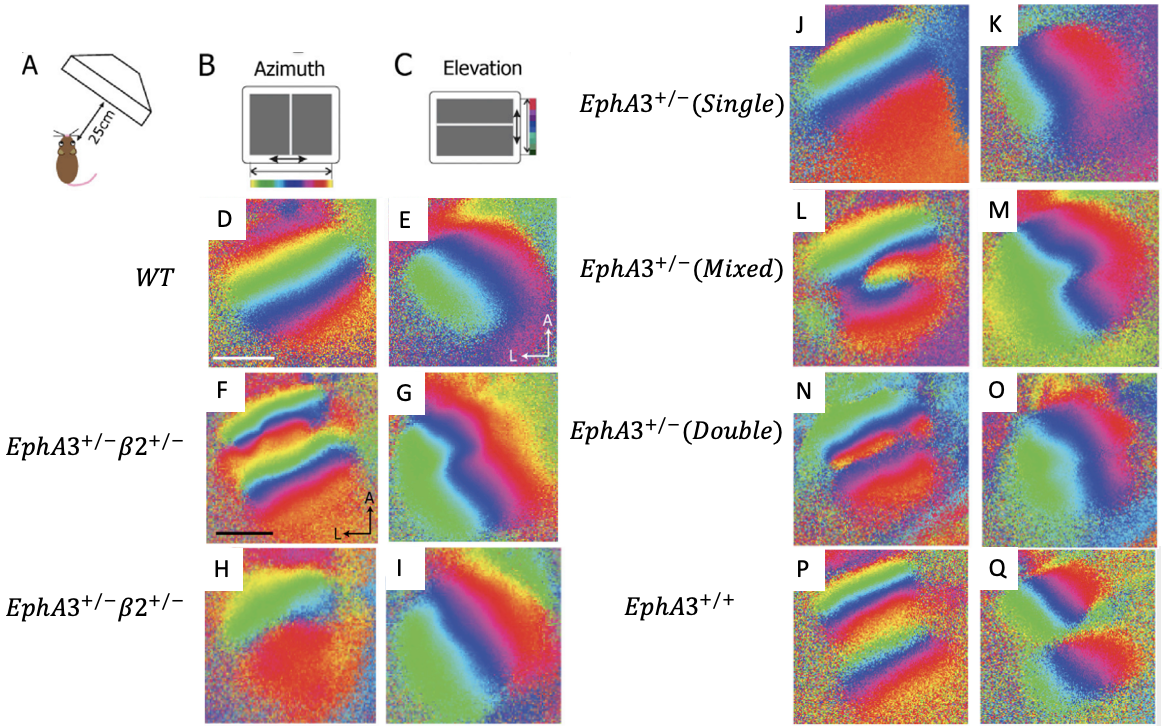
\includegraphics[width=\textwidth]{images/lattice/owenscomp}
	\def\c{The diversity of intrinsic optical imaging scans captured in the Owens et. al. (2015) dataset. }
	\caption[\c]{\c The experimental is shown in panels A-C. A representative set wild-type scans is shown in panels D and E. The scans for heterozygous EphA3 knock-in without altered neural activity patterns, EphA3$^{+/-}$$\beta2^{+/-}$, are presented in panels F and G. The EphA3$^{+/-}$$\beta2^{-/-}$ with disrupted neural activity patterns are presented in panels H and I. Representative scans of the  EphA3$^{+/-}$ heterozygote knock-in are shown in panels J-O and show phenotypes corresponding to wild-type, a mixed state, and EphA3$^{+/+}$ homozygotes. Representative EphA3$^{+/+}$ homozygote scans are shown in panels P and Q. Figure adapted from Owens et. al. (2015) \cite{Owens2015-zv}. \label{fig:owens}}
\end{figure}

\FloatBarrier
These data and observations provide several interesting challenges from a theoretical perspective with the principle question being: where is the stochasticity in the data arising from? The model is stochastic but the stochasticity is used as a minimisation technique and this does not necessarily imply stochasticity in the developmental mechanisms \cite{Tsigankov2006-uy}. Critically, the model enforces a one-to-one mapping between retinal and collicular locations which implicitly models the competitive nature of development but is arbitrarily strict and physically unrealistic. When combined with the Metropolis-Hastings methodology for energy minimisation this condition limits the search space of possible maps and can introduce artefacts not related to the underlying biology. This version of the model was later updated by Triplett et. al. (2011) to include a more realistic realisation of competition and is therefore a more appropriate theoretical tool with which to investigate this hypothesis --- this updated model was not discussed by Owens et. al. (2015) \cite{Triplett2011-jk, Owens2015-zv}. The stochastic nature of the data also provides an avenue to explore the underlying statistical properties of the model and methodologies to explore its parameter space which has not been historically done; see Section \ref{sec:koulakov}. 

The data analysis performed by Owens et. al. (2015) will be summarised followed by the reanalysis of the data done by David Willshaw which will contextualise the following modelling work \cite{Owens2015-zv}. A pipeline which is able to capture the intrinsic optical imaging process will be developed so that the recorded functional maps can be unified by with the underlying anatomy predicted by the model. This pipeline will allow the generation of lattice objects which can be compared with the biological data and also be used to generate distributions of relevant statistics to explore the principal hypothesis.
\section{Data Analysis \label{section:owensanalysis}}
The dataset generated by Owens et. al. (2015) is comprised of intrinsic optical imaging scans from 16 EphA3$^{+/-}$ mice, 5 homozygous EphA3$^{+/+}$ mice, and five wild-type mice \cite{Owens2015-zv}. The perturbations are restricted to the nasotemporal-rostrocaudal projection which varies primarily azimuthally and the original analysis accordingly generated 1-dimensional mapping profiles along this axis taken along three straight lines drawn through the colliculus which were thought to correspond with iso-elevational lines. For each of the three profiles the correlation coefficient was computed and two indexes were generated as functions of the three correlation coefficients: the linear fit index and intra-map index. These indexes were plotted against each other which revealed clustering of wild-type and homozygous specimens with the heterozygotes distributed between. There are two salient potential issues with this analysis: straight collicular lines do not correspond to iso-elevational contours and the clustering analysis indexes correlate with each other. The first issue may be resolved by realising that each of the image coordinates corresponds to a physical location which can be registered between the elevational and azimuthal scans and the elevational scan may be used to trace iso-elevational lines. The second issue may potentially not interfere with the end result but cannot be resolved.
\subsection{Reanalysis of Experimental Data \label{section:davidsresults}}
David Willshaw performed extensive reanalysis of the dataset in the context of our collaboration to complement the original analysis performed by Owens et. al. (2015) and will be summarised here. The analysis combined the elevational and azimuthal scans so that each collicular pixel had an associated coordinate in visual space thereby having a datum of the four dimensional topographic object discussed in Section \ref{sec:dimensionspace}. The colliculus region is defined by an ellipse encompassing the region where the stimulus excitation from the visual field is highest \cite{Kalatsky2003-cz}. The data then went through two filtering schemes to improve quality. First, the bulk, or average, activity was calculated for each pixel in the collicular region over the time course of the stimulation and the 10000 most active were selected. Second, the mean phase convolved over a pixel width of 5 was calculated and when the standard deviation of this mean is three times greater than the wild-type standard deviation the pixels are excluded. This step was performed because when the stimulus reaches the boundary of a functional map it will be stimulated from two distal retinal locations and thus be highly variable \cite{Willshaw2014-ms}. The phase measurement will be associated with the average position of these two distal locations and it cannot be reliably mapped to either; a problem associated with the subjectivity of the visual-collicular projective map discussed in Section \ref{section:receptivefield}. These filtering processes allow the definition of a complete map conditioned on the visual stimulus of physical collicular locations. The pixels that constitute these maps are represented in grey, and the pixels that are filtered in green. Three curves of iso-elevation are shown in the eligible grey pixels at $-25^\circ$, $0^\circ$, and $25^\circ$ which are represented in orange, cyan, and brown respectively.

With a complete representation of the topographic relationship the Lattice method of data analysis can be applied to each of these datasets discussed in Section \ref{sec:lattice}.A subset of eligible pixels with a mean spacing of 6 pixels was chosen or 80$\mu$m to tile the colliculus. The spacing between collicular nodes was chosen to be the smallest that gives highly ordered 2D maps in wild-types, as found in an analysis of another data set \cite{Willshaw2014-ms}. The mean visual field of all pixels falling with 3 pixels of these locations was calculated and associated with each location. The tiling was projected to the visual field and any edges found to be crossing were removed and highlighted in red with the resulting map giving a standardised topographic representation of the data: a lattice object. In the case of the heterozygotes and homozygotes and the data may be further subdivided into rostral and colliculus portions by creating a partitioning line through the excluded high variance points (green). This line was fitted by visual examination. Each of these regions can be associated with a part-map or lattice object constructed from pixels only in this region. An example of the lattice object generated for a wild-type is shown in Figure \ref{fig:wild-type1}. The variation in the iso-elevational lines indicates a marginal distortion in the dorsal-ventral axes.  

\begin{figure}
	\centering
	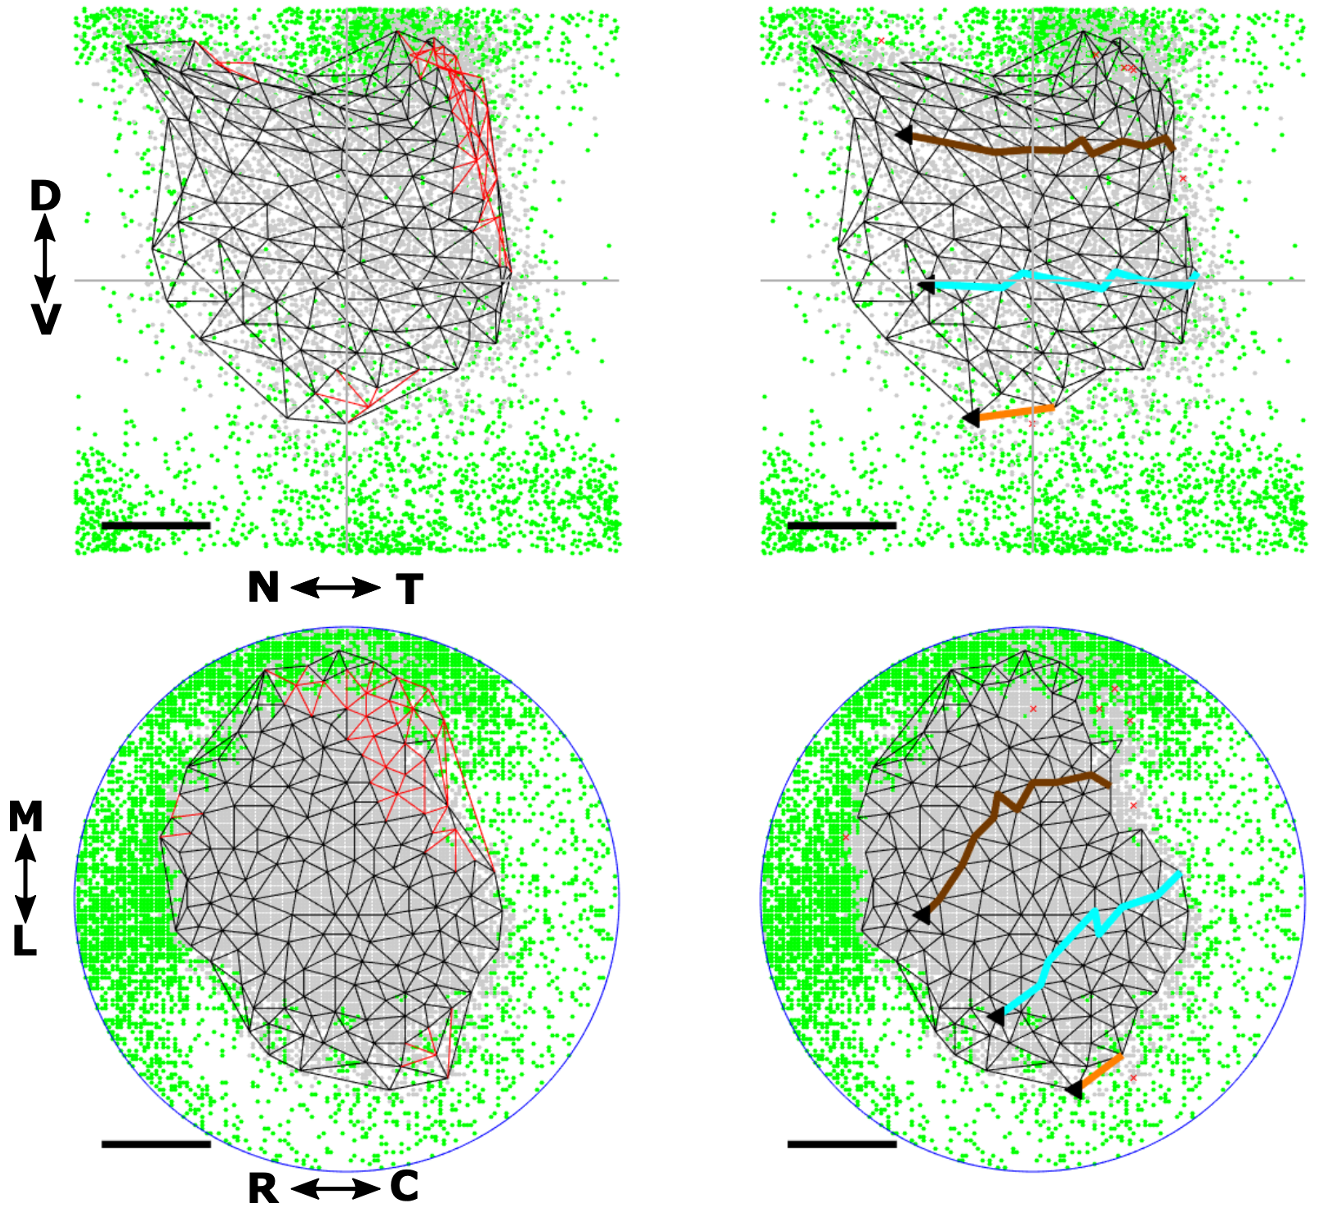
\includegraphics[width=\textwidth]{images/lattice/figwt}
	\def\c{An example of a lattice generated from a wild-type dataset. }
	\caption[\c]{\label{fig:wild-type1}\c The scale bar is 200um. There are several conventions in the image worth outlining. First, the green pixels are filtered data while the grey indicates the retained data. Second, the whole map is presented to the left conventionally while the largest ordered submap is presented to the right. The excluded links are highlighted in red in the original map and have a corresponding red cross on the submap. The three iso-elevational lines are represented in brown, cyan and orange. This example represents an excellent local ordering as only 4\% of the nodes had to be removed to give the largest ordered submap and high polarity scores. Figure reproduced from Willshaw and Gale (2022) \cite{Willshaw2022-fs}.}	
\end{figure}

For each dataset the lattice objects were to calculate a series of statistics and the following are chosen for this thesis: azimuthal and elevational magnification, map quality, and visual field overlap. Magnification ratio is a measure of the relative extent of the projection along a specified axis. The Azimuthal Magnification (AM) is the length of each edge measured along the rotated nasotemporal axis of visual field compared to the length of the corresponding edge along the rostrocaudal axis of the colliculus; similarly for the Elevational Magnification but this is of less interest in genotypes with disrupted A-system signalling.  Map quality refers to the number of nodes which need to be removed in order to form the perfect topographic representation. In cases when two maps were constructed by partitioning the colliculus, the extent of visual field which projects to both regions of the colliculus, called the Visual Field Overlap (VFO), was measured. In a complete double map, the VFO is the entire extent of visual field. These statistics were used to classify the heterozygotes into three categories concordant with the Owens et. al. analysis: HETA, HETB, and HETC. Example maps for these three heterozygote categories are shown in Figure \ref{fig:examples}.

The statistics associated with each population are shown in Table \ref{table:lattticestats}. The HETA classification shows very similar statistical profiles to the wild-type with no visual field overlap being recorded. The HETB specimens are beginning to deviate particularly in VFO. The HETC specimens present more similarly to HOM specimens with similar VFO and map qualities. The azimuthal magnification is distinguished between the two part maps due to the compression of each map into a region of the colliculus. The elevational magnification remains unchanged. The Lattice method has revealed evidence for two part maps in all of the homozygotes and to a lesser degree each of the heterozygotes. These part maps are formed by bisecting the colliculus into two regions on the basis of data quality and when this bisection is made each of the part maps form individual higher quality lattices than the whole map lattice. These higher quality maps can be used to interrogate the coverage of the visual field and in particular the overlap of the visual space covered by each part map: the VFO. 
\begin{table}[h!]
	\centering
	\begin{tabular}{|c|c c c c c|}
	\hline
	\textbf{Statistic}  & Wild Type & HETA & HETB & HETC & Hom\\
	\hline
	Whole Map AM & $1.54  \pm -$ & $0.93 \pm 0.13$ & $1.03 \pm 0.11$  & $1.11 \pm 0.12$ & $1.49 \pm 0.2$ \\
	Rostral AM & $- \pm -$ & $0.26 \pm 0.36$ & $1.16 \pm 0.1$  & $1.34 \pm 1.34$ & $2.03 \pm 0.2$ \\
	Caudal AM & $- \pm -$ & $0.41 \pm 0.57$ & $0.81 \pm 0.07$  & $ 0.75 \pm 0.75$ & $1.03 \pm 0.27$ \\
	Whole Map Quality & $91 \pm 4$ & $86 \pm 2$ & $91 \pm 5$  & $78 \pm 19$ & $71 \pm 10$ \\
	Rostral Quality & $- \pm -$ & $- \pm -$ & $97 \pm 1$  & $93 \pm 6$ & $91 \pm 6$ \\
	Caudal Quality & $- \pm -$ & $- \pm -$ & $88 \pm 9$  & $89 \pm 8$ & $90 \pm 15$ \\
	VFO& $- \pm -$ & $0 \pm 0$ & $5 \pm 2$  & $ 27 \pm 13$ & $33 \pm 18$ \\
	\hline
	\end{tabular}
	\def\c{Summary statistics based on the lattice analysis. }
	\caption[\c]{\c The magnification ratios for each of the part maps are summarised (where appropriate) with the rostral projection and the caudal projection is reported in parenthesis and square brackets respectively. The whole map quality is shown to degrade from wild-type to homozygote and the average part map quality is reported in parenthesis and square brackets respectively. The VFO increases from wild-type to homozygotes. The VFO and map quality statistics appear to be the most relevant statistics to query whether there is a significant overlap between classifications. These statistics are generated on small samples (~5 specimens each) and caution should be applied interpreting them. \label{table:lattticestats}}
\end{table}
\begin{landscape}
\begin{figure}[h!]
	\centering
	\begin{subfigure}{0.75\textwidth}
		\centering
		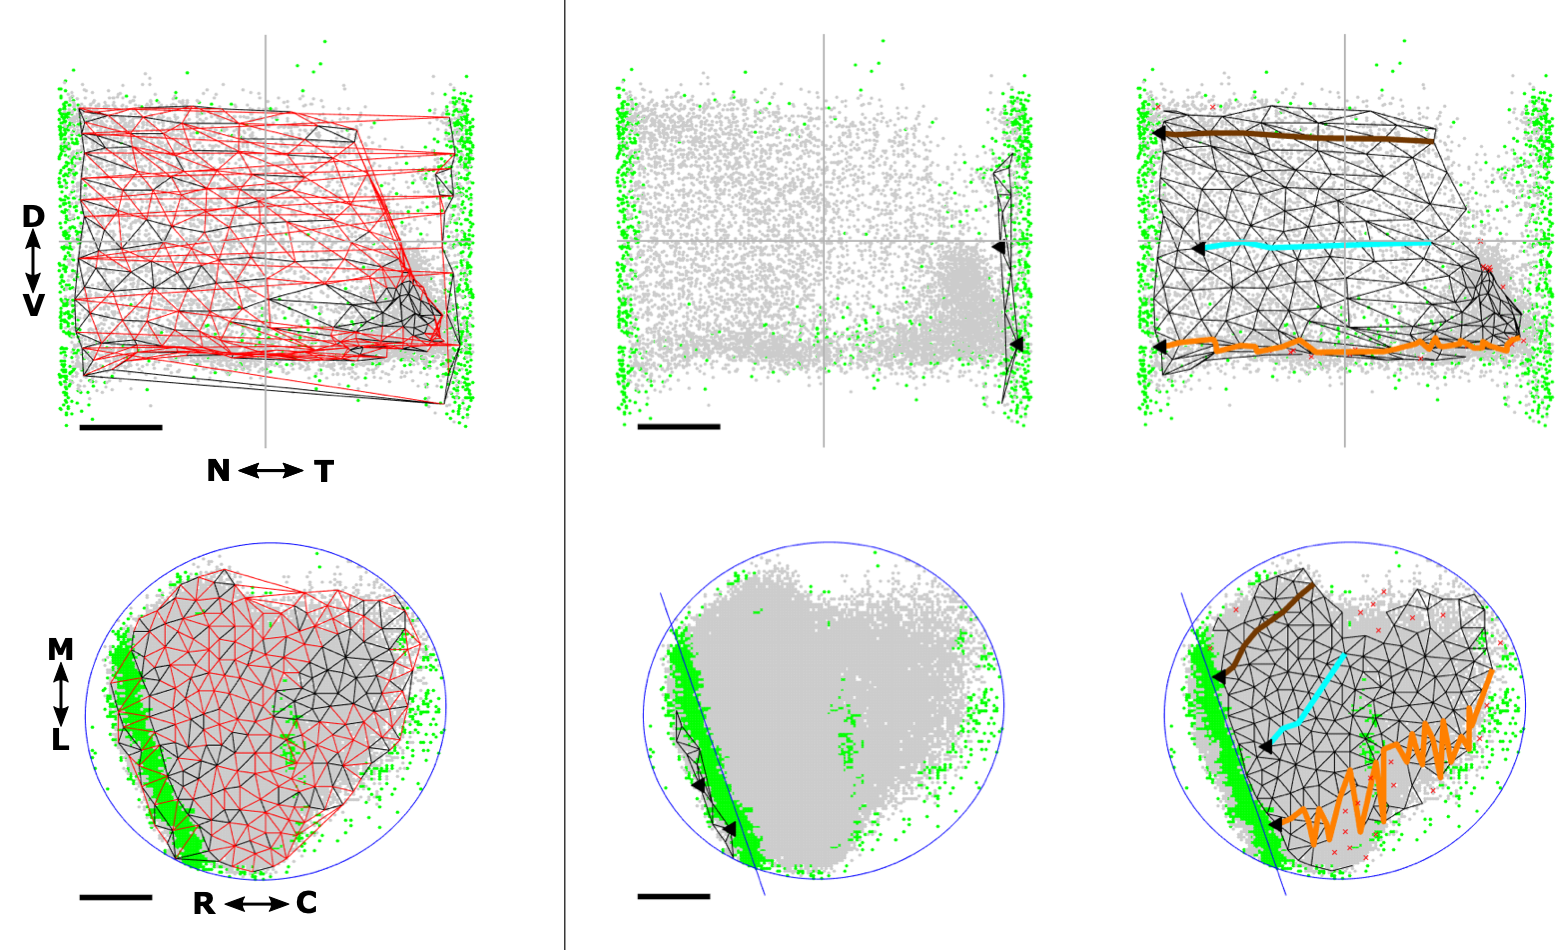
\includegraphics[width=\textwidth]{images/lattice/figHETA1}
		\caption{\textbf{HETA}}
	\end{subfigure}
	~
	\begin{subfigure}{0.75\textwidth}
		\centering
		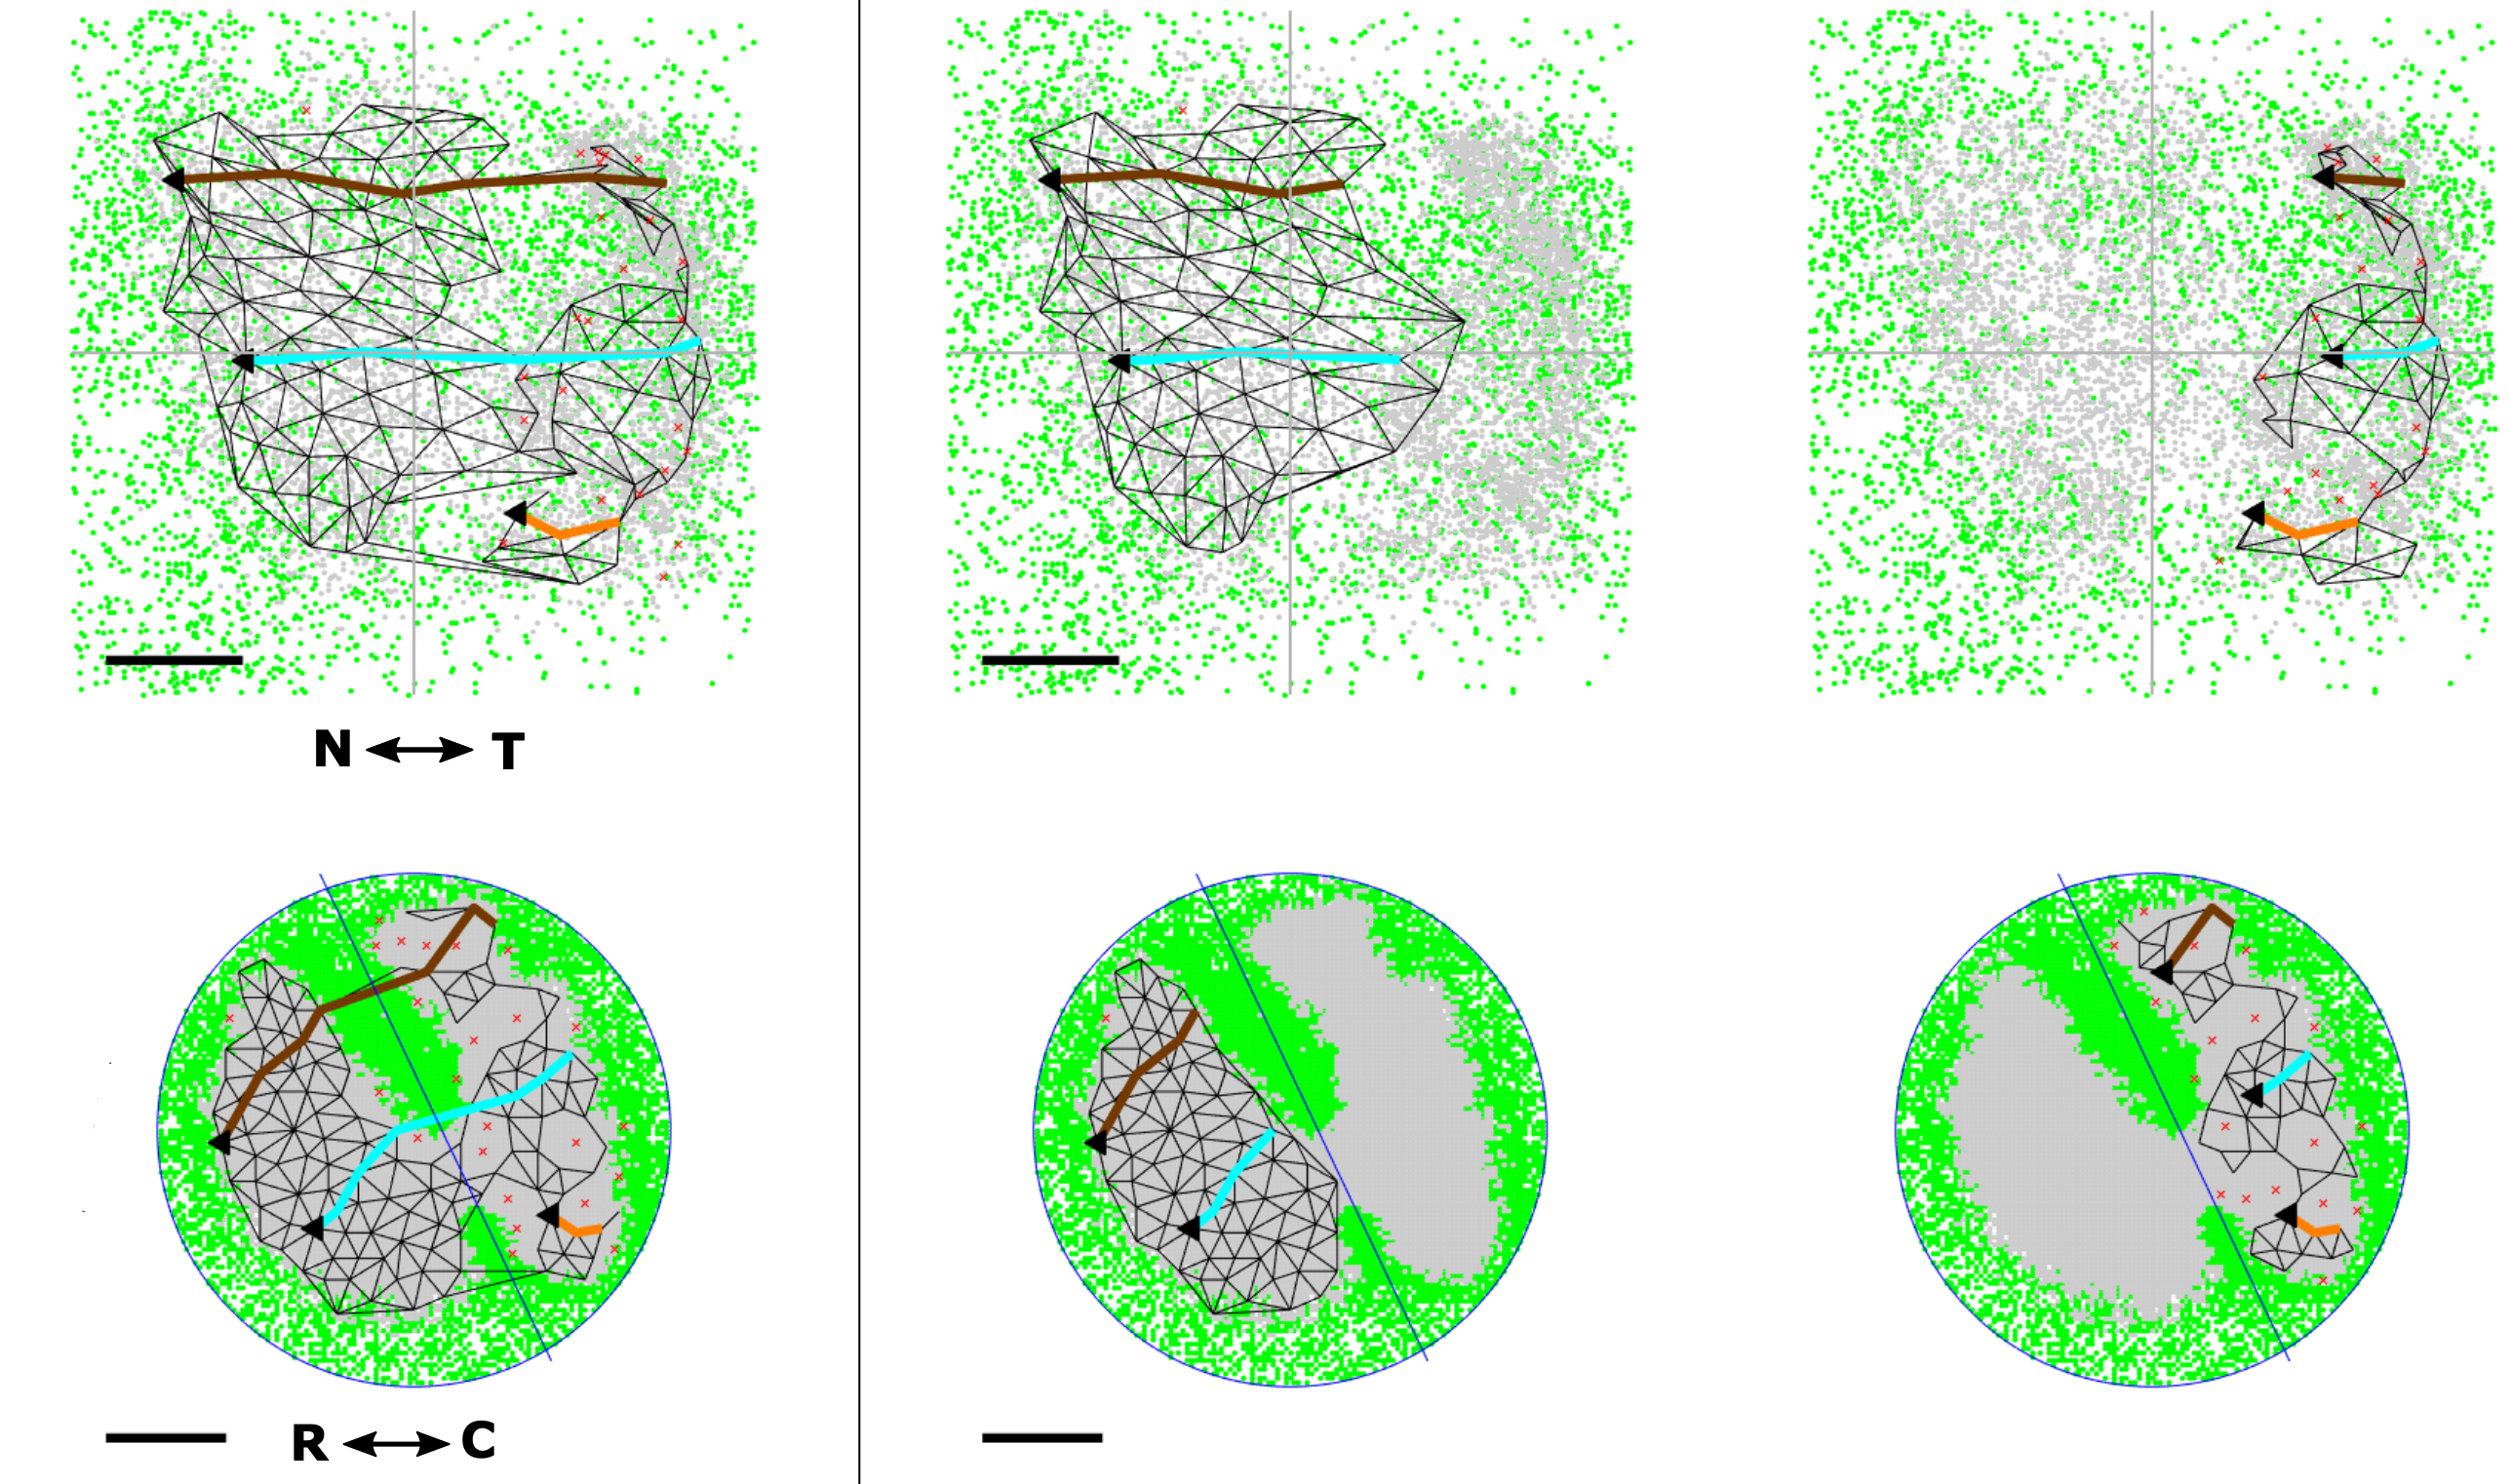
\includegraphics[width=\textwidth]{images/lattice/figHETB1}
		\caption{\textbf{HETB}}
	\end{subfigure}
	
	\begin{subfigure}{0.75\textwidth}
		\centering
		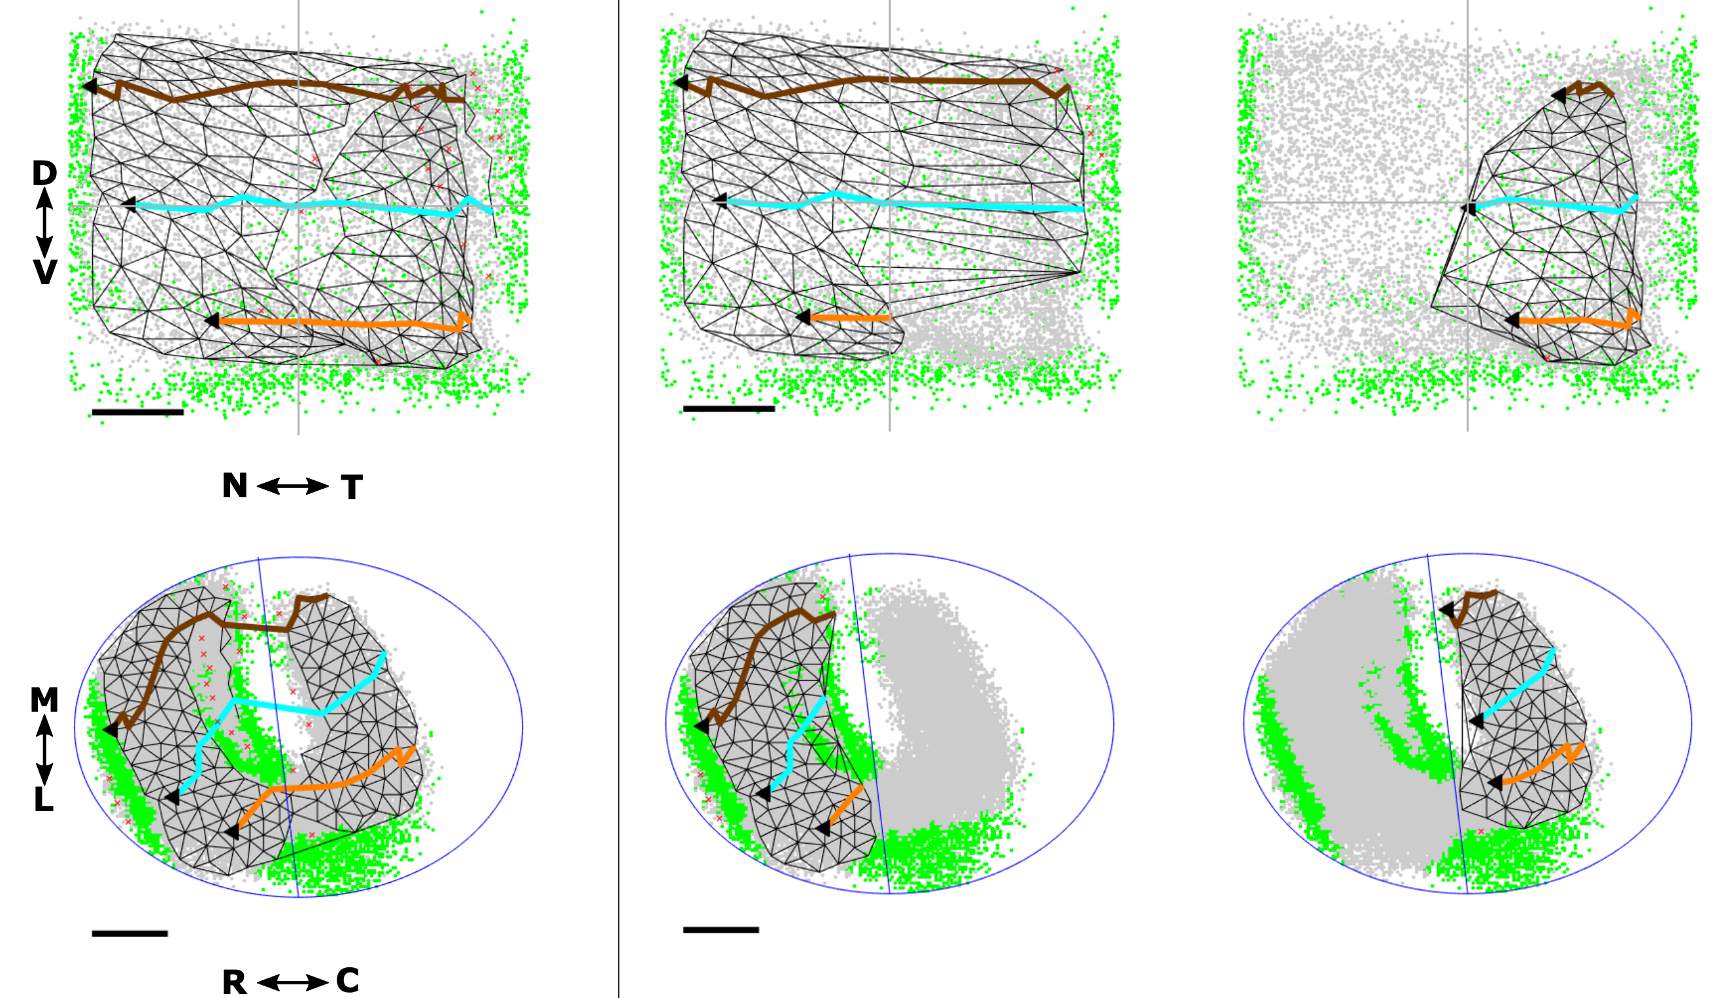
\includegraphics[width=\textwidth]{images/lattice/figHETC2}
		\caption{\textbf{HETC}}
	\end{subfigure}
	~
	\begin{subfigure}{0.75\textwidth}
		\centering
		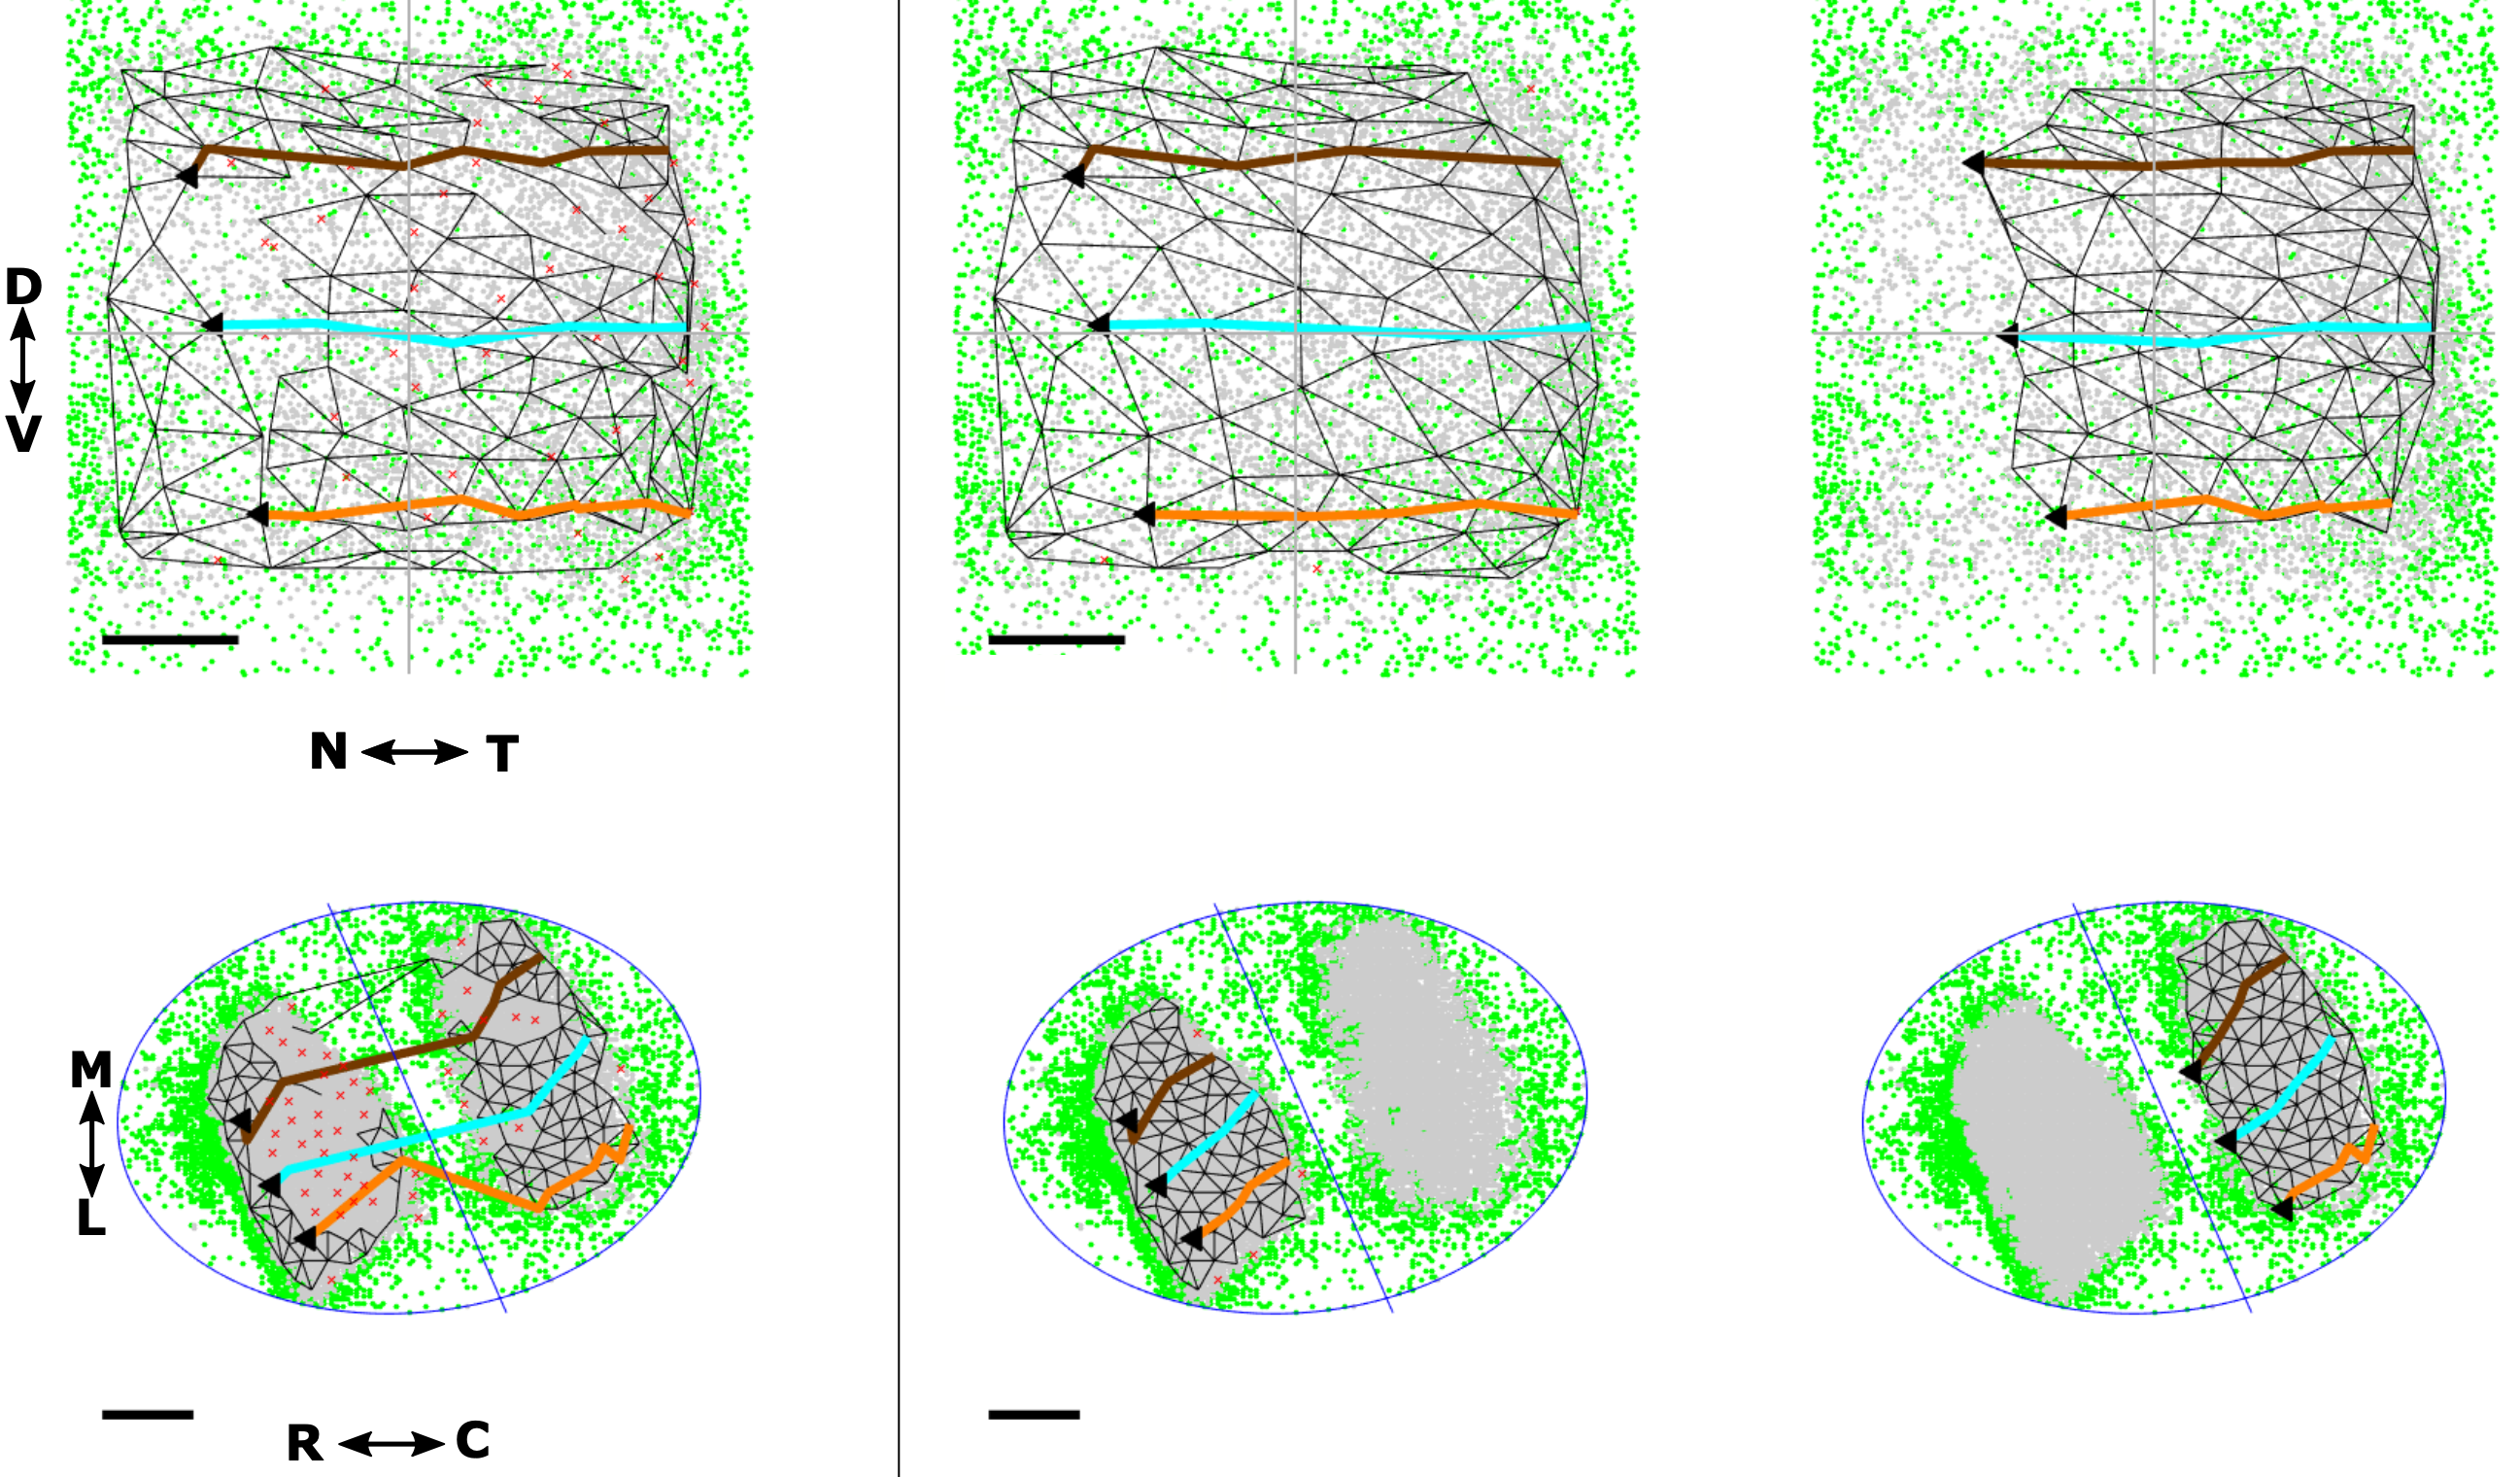
\includegraphics[width=\textwidth]{images/lattice/figHOM2}
		\caption{\textbf{HOM}}
	\end{subfigure}
\end{figure}
\end{landscape}
\addtocounter{figure}{-1}
\begin{figure}[h!]
\def\c{Examples for the three heterozygous classifications and the homozygous maps. }
\caption[\c]{ \c For each of these maps the whole map lattice is calculated and shown in the left and the rostral and caudal part-maps are shown on the right; the scale bar is 200um.. An example map for the A classification is shown in panel (a) and shows a very small secondary part map with reversed polarity. When the two part-maps are disambiguated the map quality improves with less nodes being removed compared to the whole map and the first part map corresponds well to a wild-type. An example map for the B classification is shown in panel (b) and while the whole map suggests a degree of ordering it is improved by separating the projection at the neck of the eligible pixels in grey. An example map for the C classification is shown in (c) and here map quality is substantially improved by segregation with a complete visual representation rostrally and a partial visual representation caudally; these heterozygotes are qualitatively similar to homozygotes in this respect. An example map of a homozygote is shown in (d) with the eligible pixels completely forming two independent regions and with each of these regions containing a well ordered and substantial portion of the visual field. Figure reproduced from Willshaw and Gale (2022) \cite{Willshaw2022-fs}. \label{fig:examples}}
\end{figure}
\section{Modelling Pipeline}
To theoretically analyse the stochastic hypothesis there needs to be a method to directly compare model output with data elements. There are two key issues here: registration and anatomical interpretation. The lattice method provides a good solution to the first problem as it is defined topologically and therefore lattice properties such as visual field coverage can be compared between two model runs without needing to ensure that all points are metrically registered against each other. The method also allows for direct comparison to the data under the hypothesis that the model generates comparable data-types. This leads to the second problem which is how the Tsigankov-Koulakov connections are precisely defined. The most reasonable interpretation given the data used to define the models is that they are anatomical, not functional \cite{Tsigankov2006-uy, Koulakov2004-ia, Tsigankov2010-on, Triplett2011-jk}. For the wild-type phenotype the distinction is irrelevant because the functional imaging scans would be in correspondence with the anatomical retinotopy. However, when there is a duplicated or ectopic connection this association is non-trivial. The phase of the signal will be now composed of several components of the visual field and the measured phases is the average phase of these components.

To compare the model and data the model is used as a network generator on which activity dynamics can be explored. The activity induced by the optical imaging paradigm can then be simulated and used to generate lattice objects which are comparable to data. This interpretation confers an additional benefit: the underlying anatomical properties of the network are completely known. Therefore anatomical lattices can be generated to make predictions about the underlying structure of maps. This is of particular interest in a related hypothesis: do the wild-type and EphA3$^{+/+}$ afferents completely segregate in the colliculus? A review by Cang and Feldheim (2013) implies that they do but this appears to be based on functional optical imaging scans while anatomical injection studies are too sparse \cite{Cang2013-dw}. These questions are intimately related to the role of competition with respect to gradient sensing mechanisms and therefore the choice of model is the Tsigankov-Koulakov model extended to have multiple connections and a competitive sorting mechanism \cite{Triplett2011-jk}. 

The anatomical model can be used as a blueprint retinotopic map on which to simulate neural activity which can be used to generate \textit{in silico} optical imaging scans. The lattice method can be used to generate statistics on this distribution of scans and thus directly compare with experimental data. The statistics of most interest for examining the heterozygote variability hypothesis are the VFO and map quality.  These two statistics can be used to classify the heterozygous variability under the following criteria: the part-map subdivision must not substantially improve map quality over the whole map to be classified as similar to wild-type and the VFO must be statistically similar to the homozygous distribution to be classified as a homozygote. 
\subsection{Anatomical Model}
The Tsigankov-Koulakov model shall be briefly covered here and it is detailed in full in Section \ref{sec:models}. The model is an energy minimization model which assigns energy to a configuration of synaptic connections between a set of collicular and retinal cells. The energy is given by:
\begin{align}
&E = E_{\text{chem}} + E_{\text{act}}+E_{\text{comp}}\\	
&E_{\text{chem}} = \sum_{p \in \{\alpha,\beta\}}\sum_{i \in \text{syn}} pR(i_\text{ret},p)L(i_\text{col},p) \\
&E_{\text{act}} =- \frac{\gamma}{2} \sum_{i \in \text{syn}}\sum_{j \in \text{syn}} C(d_R(i, j))U(d_C(i, j)) \label{eq:latticemodelequation}\\
&E_{\text{comp}} = \sum_{i\in \text{ret}} (n_i^2 - 500 n_i^{1/2}) + \sum_{i\in \text{col}} n_i^2.
\end{align}
The chemotactic term is given with $\alpha=-90$ $\beta=120$ with the change in sign indicating that the B system is attractive and the A system repulsive, $R$ and $L$ are the masked gradients (the difference between Eph and ephrin levels) in retina and SC locations respectively, and the sum is performed over all possible synapses; the parameters and gradients are inherited from previous iterations of the model. It is important to note that this masking ensures that the system is a Type I or graded matching. The activity term is the sum over all pairs of synapses of the product of two correlation functions which take the normed distance between a synapse pair in the retina, $C(d_R) = \exp(-|d_R|/11)$, and colliculus, $U(d_C) = \exp(-d_C^2/18)$, where the $d_R$ and $d_C$ are the metric functions for the retina and colliculus respectively and the parameters $11$ and $18$ and $\gamma=0.00625$. Finally, the competition term is given by two sums: one over over the SC and retinal locations. The sums compute the square of the number of synapses for the SC sites, and the difference between square and square root of the number of synapses for the retinal sites. In this fashion, it is energetically favourable to have some, but not too many, synapses between locations. The forms and parameters of the function are chosen arbitrarily.

The minimisation procedure involves the creation and deletion of synapses. At each simulation time-step a potential pairing of an SC and retinal site is considered and the change to the energy function that adding this site would induce is calculated. A uniform random number $u$ is generated and compared to:
\begin{equation}
p = \frac{1}{1+\exp(-4\Delta E)},
\end{equation}
and the change is accepted if $p<u$ thus promoting changes which lower the energy whilst stochastically accepting higher energies infrequently. The same procedure is repeated except sampling amongst existing synapses and preferentially deleting synapses which contribute high energy. The model was allowed to run for $5\times N^2$ time-steps where N is the number of cells in the colliculus and retina. The parameter choices made here follow the paper and Git repository for Hjorth (2015) \cite{Hjorth2015-le}. These parameters have produced good results in this study but it is still prudent to exercise caution about them given that there are no comprehensive studies exploring the parameter space of this model.

For high resolution maps the number of cells was chosen to be $N = 10000$ (in line with the number of active pixels in the data analysis) while for low resolution maps which converged quickly the number of cells was $N = 2000$. The model was implemented computationally using the MATLAB package developed by Hjorth et. al. (2015) \cite{Hjorth2015-le} on am AMD Ryzen Threadripper 3950X with 32 cores.

To model the EphA3 systems a fraction of retinal cells were chosen to be tagged as EphA3$^{+/-}$ cells. This fraction was typically 50\% but fractions of 40\% and 50\% were also examined. To each of these tagged cells an additional $\Delta R$ was added to their EphA level given by their position `$x$' in the EphA gradient $R_A(x)$. The gradients are normalised to a maximum value of one in the wild-type and it remains an open question what $\Delta R$ should be equal to. It seems reasonable that the homozygote should be twice that of the heterozygote but this does not follow automatically. In light of these considerations, a parameter sweep of $\Delta R$ was performed to understand its effects in parameter space more generally. The codebase used to perform the following simulations is freely available online \cite{LatticeEphA3}.
\newpage
\subsection{Spiking Model of Neural Activity}
To simulate activity in the superior colliculus a simple Poisson integrate-and-fire model was chosen; see Section \ref{sec:activity}. It was assumed that each collicular $i$ cell is connected to each retinal cell $j$ with a weight $W_R(i,j)$ given by the output of the anatomical model, and to other collicular cells $k$ with a weight given by the function of the distance $d_{ik}$ between them:
\begin{equation}
W_C(i, k) = w_1 \exp\left(-\frac{d_{ik}^2}{2r_1^2}\right) -w_2 \exp\left(-\frac{d_{ik}^2}{2r_2^2}\right),
\end{equation}
where the colliculus length was normalised to one and $r_1 = 0.01, r_2 = 0.02, w_1 = 0.02$, and $w_2 = 0.01$ to mimic the lateral connectivity pattern reported in the colliculus \cite{Phongphanphanee2014-in}. These are first order approximations of the recurrent kernel which differ from the estimates given in Chapter \ref{chapter:neuralstdp}. This is due to the slightly different geometries employed in each model. Each collicular cell receives input in the form of spikes from retinal cells and other collicular cells and these spikes are integrated over time to form the rate parameter:
\begin{equation}
r_i(t, t_0) = \int_{t0}^t dt \left( \frac{1}{\sum_jW_R(i,j)}\sum_{j} W_R(i,j) I_R(j, t) + \frac{1}{\sum_kW_C(i,j)}\sum_{k} W_C(i,j) I_C(k, t) \right),
\end{equation} 
where $t_0$ is the time of the last collicular spike in collicular cell $i$, and $I_R(j,t)$ and $I_C(k, t)$ are the spike trains for retinal index $j$ and collicular index $k$ respectively. The sampling rate was set at $dt = 0.01$ seconds and at each timestep $dt$ a random number $p_i$ was drawn and a spike generated in collicular index $i$ if:
\begin{equation}
r_i(t, t_0) dt < p_i.
\end{equation}
A record of all collicular spikes was generated and associated with collicular activity generated by stimulating the retina with a given input pattern, $I_R(j, t)$, chosen to represent the experimental paradigm described in Section \ref{section:OIS}. 
\newpage
\subsection{Optical Image Scan Reconstruction \label{section:OIS}} 
To reconstruct the optical images the procedure outlined by Kalastky and Strkyer (2003) was replicated \cite{Kalatsky2003-cz}. A wave of stimulus was applied across the retina as input in an orthogonal direction repeated with periodic boundary conditions ten times. The activity is propagated into the network model as a series of neuronal spikes generated by a Poisson process and this combined with lateral connectivity generates a series of spikes in the colliculus. The procedure is reversed and two records of the activity in the forward and reverse directions are kept. The entire procedure is again repeated along the complementary orthogonal direction and these are associated with azimuthal and elevational activity. Figure \ref{fig:activitydem} shows the phase plots for a wild-type phenotype, Figure \ref{fig:scans} shows the azimuthal phase plots for heterozygous and homozygous knock-ins. The lattice method can be applied directly to this surrogate phase data and forward (visual field to colliculus) and reverse (colliculus to visual) field are shown conventionally in blue and black respectively; see Figure \ref{fig:wholemap}.
\begin{figure}[h]
	\begin{subfigure}{0.5\textwidth}
		\centering
		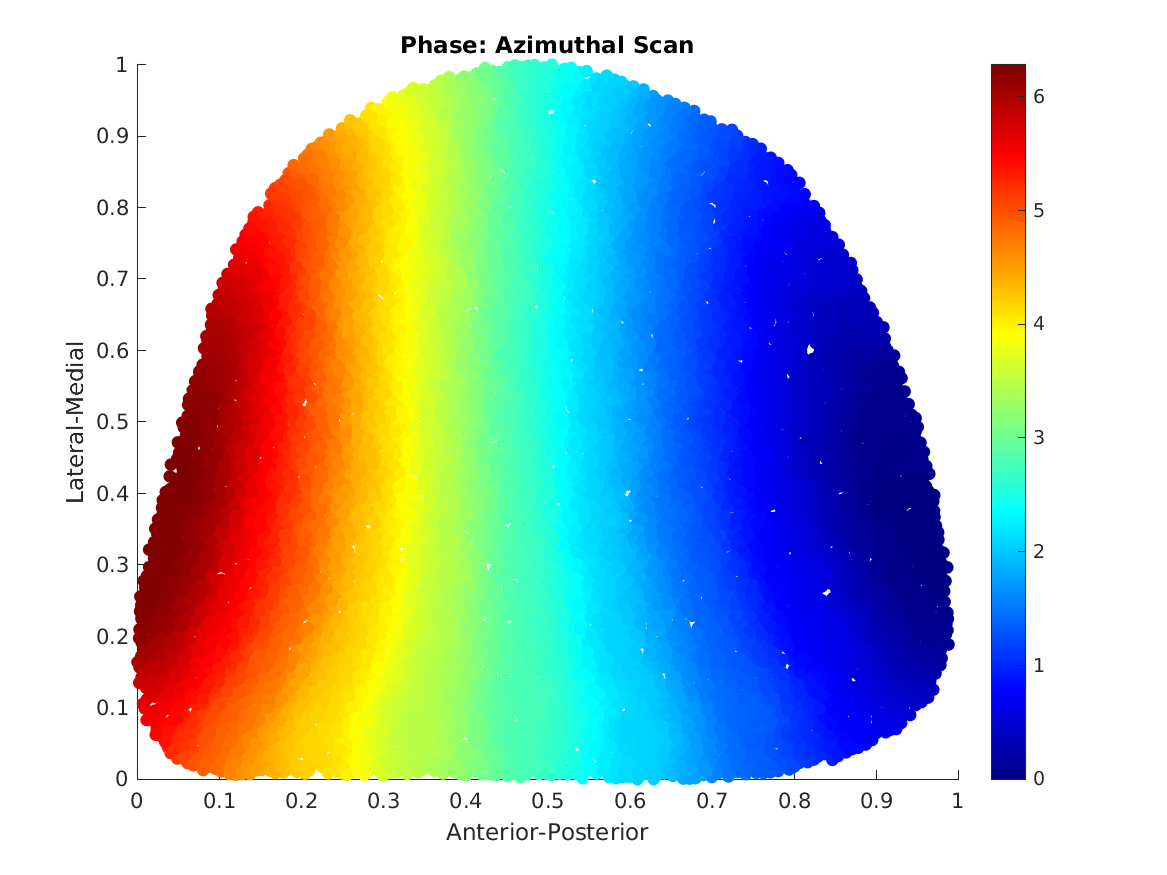
\includegraphics[width=\textwidth]{images/lattice/WT1}
		\caption{}
	\end{subfigure}
	\begin{subfigure}{0.5\textwidth}
		\centering
		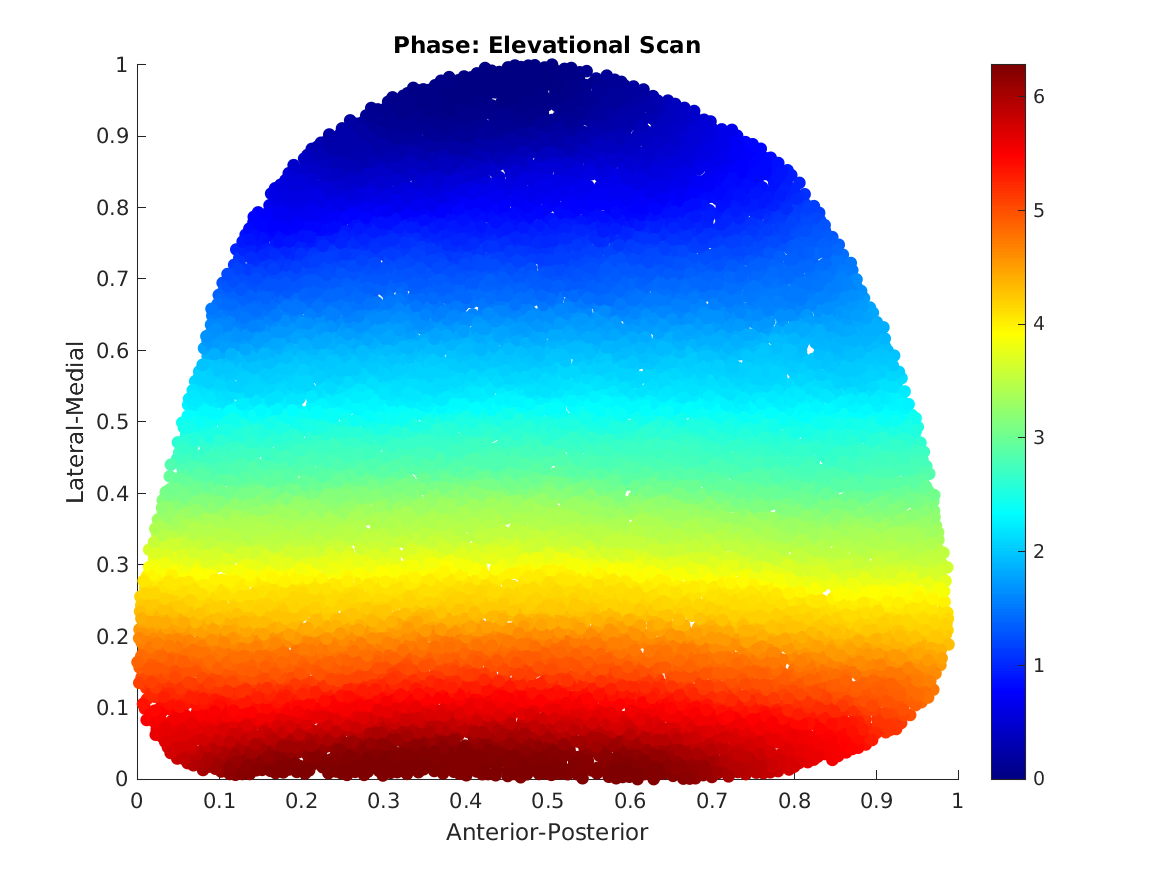
\includegraphics[width=\textwidth]{images/lattice/WT2}
		\caption{}
	\end{subfigure}
	\def\c{The azimuthal and elevational phase diagrams for a wild-type simulation. }
	\caption[\c]{The azimuthal and elevational phase diagrams for a wild-type simulation are presented in panels (a) and (b) respectively following the procedure outlined Kalatsky and Stryker (2003) \cite{Kalatsky2003-cz}. There is a good correspondence between these phases maps and those measured biologically. It is important to note that biological phase maps are stimulated azimuthally and conventionally and these roughly correspond with the orthogonal gradients in the retina but not precisely, in these maps this relationship is precise but the naming convention is kept.} \label{fig:activitydem}
\end{figure}
\FloatBarrier
	
\begin{figure}[h]
~\unskip\ \vrule\ 
~\unskip\ \hrule width0.985\textwidth
~\unskip\ \vrule\ 
	\begin{subfigure}{0.47\textwidth}
		\caption{Colliculus to Field: Whole Map}
		\centering
		\includegraphics[width=0.95\textwidth]{images/lattice/example_lattice_CTOF_whole}
	\end{subfigure}
~\unskip\ \vrule\ 
	\begin{subfigure}{0.47\textwidth}
		\caption{Colliculus to Field: Part Maps}
		\centering
		\includegraphics[width=0.95\textwidth]{images/lattice/example_lattice_CTOF_sub}
	\end{subfigure}
~\unskip\ \vrule\ 
~\unskip\ \hrule width0.985\textwidth
~\unskip\ \vrule\ 
	\begin{subfigure}{0.47\textwidth}
		\caption{Field to Colliculus: Whole Map}
		\centering
		\includegraphics[width=0.95\textwidth]{images/lattice/example_lattice_FTOC_whole}
	\end{subfigure}
~\unskip\ \vrule\ 
	\begin{subfigure}{0.47\textwidth}
		\caption{Field to Colliculus: Part Maps}
		\centering
		\includegraphics[width=0.95\textwidth]{images/lattice/example_lattice_FTOC_sub}
	\end{subfigure}
~\unskip\ \vrule\ 
~\unskip\ \hrule width0.985\textwidth
~\unskip\ \vrule\ 
	\def\c{A series of whole maps and part-maps generated on anatomical data for a simulation ($\Delta R = 0.565$). }
	\caption[\c]{\c Each panel has four lattices with the top two corresponding to retinal nodes and the bottom to corresponding to collicular nodes. The black lattices in panel A are constructed using the colliculus as the pre-image and represent the lattice object generated on the entire set of collicular nodes. The whole map lattice is presented on the left of panel A and the largest submap on the right with excluded links highlighted in red. The black lattices in panel B are the largest submap lattices constructed on the rostral and caudal nodes in the colliculus. To construct each of these submaps a partitioning line is created at the average rostrocaudal location of the filtered (green) nodes and the rostral partmap is constructed using collicular points left of this line and the rostral partmap using the points right of the line. The blue lattices in panel C are the whole map lattices as in Panel A but constructed using the retina as the pre-image in the Lattice Method. The lattices in panel D are part map lattices that are constructed using the $Islet2$ expressing cells (left partmap) and $Islet2$ non-expressing cells (right partmap); since both populations are relatively uniformly expressed on the retina the pre-image lattice has good retinal coverage which differs to the pre-image coverage of the collicular partmaps in B. Each of the partmap projections have an overlap which is highlighted in purple; this overlap for a collicular pre-image (black) corresponds to the VFO. This example highlights how carefully partitioning the colliculus (or retina) carefully can reveal well ordered properties that would not be measurable by analysing the map as a whole. \label{fig:wholemap}}
\end{figure}
\FloatBarrier
\section{Results}
The value of $\Delta R$ to generate a heterozygous or homozygous genotype is not known \textit{a priori} and therefore a range of values $\Delta R = \{0.0565 i\}_{i=0}^{i=10}$ was interrogated; this is analogous to assuming a uniform prior on the $\Delta R$ parameter. Several anatomical experiments are performed on these maps, followed by a lattice analysis, before attempting to analyse the statistical properties of these maps at a lower but more computationally manageable resolution.
\subsection{Anatomical Experiments}
The model allows the provenance of a synaptic connection to be recorded: a synapse's origin can be labelled as an EphA3 expressing or wild-type cell in the retina. In the following experiments this is exploited by labelling wild-type cells in red and EphA3 tagged cells in gold. 

Anterograde dye injections into the retina are made to stain the colliculus. From these the average projection location in the rostrocaudal of all cells within a given tolerance of 1\% in the nasal-temporal axis is calculated. The analogous retrograde injection into the colliculus to stain the retina is also performed. These simulations reproduce in a single map the experimental injections performed and averaged over many mice \cite{Brown2000-da}. The results are in accordance with those experiments demonstrating that the model predicts individual map presentations correlate closely with aggregate population maps. These experiments can be seen in the third and fourth rows of Figure \ref{fig:antomicalEphA3}.

Next, the whole retina was flooded with red and gold labelled dyes in an experiment analogous to the one performed for the $Math5^{-/-}$ mutant \cite{Triplett2011-jk}. This experiment reveals the area of the colliculus which each cell type is restricted to and is useful to provide a register for the domains of each cell type. For low amounts of $\Delta R$ the populations are fairly well mixed across the colliculus and become increasingly segregated with an increasing level of $\Delta R$. For the maximum observed level of $\Delta R=0.56$ the maps become completely almost completely segregated with a slight overlap. These experiments can be seen in the final row of Figure \ref{fig:antomicalEphA3}.
\begin{landscape}
\begin{figure}
	\centering
	\includegraphics[width=1.6\textwidth]{images/lattice/paper_anatomy_dr}
	\def\c{A series of injection experiments are performed on knock-in simulations with $\Delta R$ increasing left to right from $\Delta R=0$ (wild-type) to $\Delta R=0.565$ (HOM). }
	\caption[\c]{\c In each plot the EphA3 projection and cell-type is labelled in gold while the wild-type cell-type is labelled in red. The first row represents the average projection from collicular cells in the rostrocaudal axes to the nasal-temporal axes (colliculus-to-field), the second represents the average projection of the retinal cells into the rostrocaudal axis (field-to-colliculus), and the third represents the retinal providence of each collicular cell. In the colliculus a number of points are highlighted in blue and these correspond to an injection made of 1\% of the retina in the central field corresponding to the experiments performed by Brown et. al. (2000) \cite{Brown2000-da}.} \label{fig:antomicalEphA3}
\end{figure}
\end{landscape}
\subsection{Lattice Analysis}
The anatomical map for each sample of $\Delta R$ was used to perform an optical imaging experiment and example azimuthal scans are presented in Figure \ref{fig:scans}. After performing the same data filtering procedure used on the biological specimens a number of different lattice objects were generated on both the anatomical and functional maps. The lattices in both directions between visual field/retina and colliculus were generated. The the average rostrocaudal location of the filtered data was used to generate a discriminator to separate the two functional colliculus maps. The collicular cells in these regions where then used to generate a lattice onto the retina to give an indication of the quality of each of the functional maps. An analogous experiment in the retina was also performed whereby the mapping was restricted to a single cell type and another scan performed to generate the lattice that this cell restricted retina would have in the absence of interactions the other cell-type; the additional scan is necessary to remove these interactions.
\begin{figure}[h]
	\begin{subfigure}{0.45\textwidth}
		\centering
		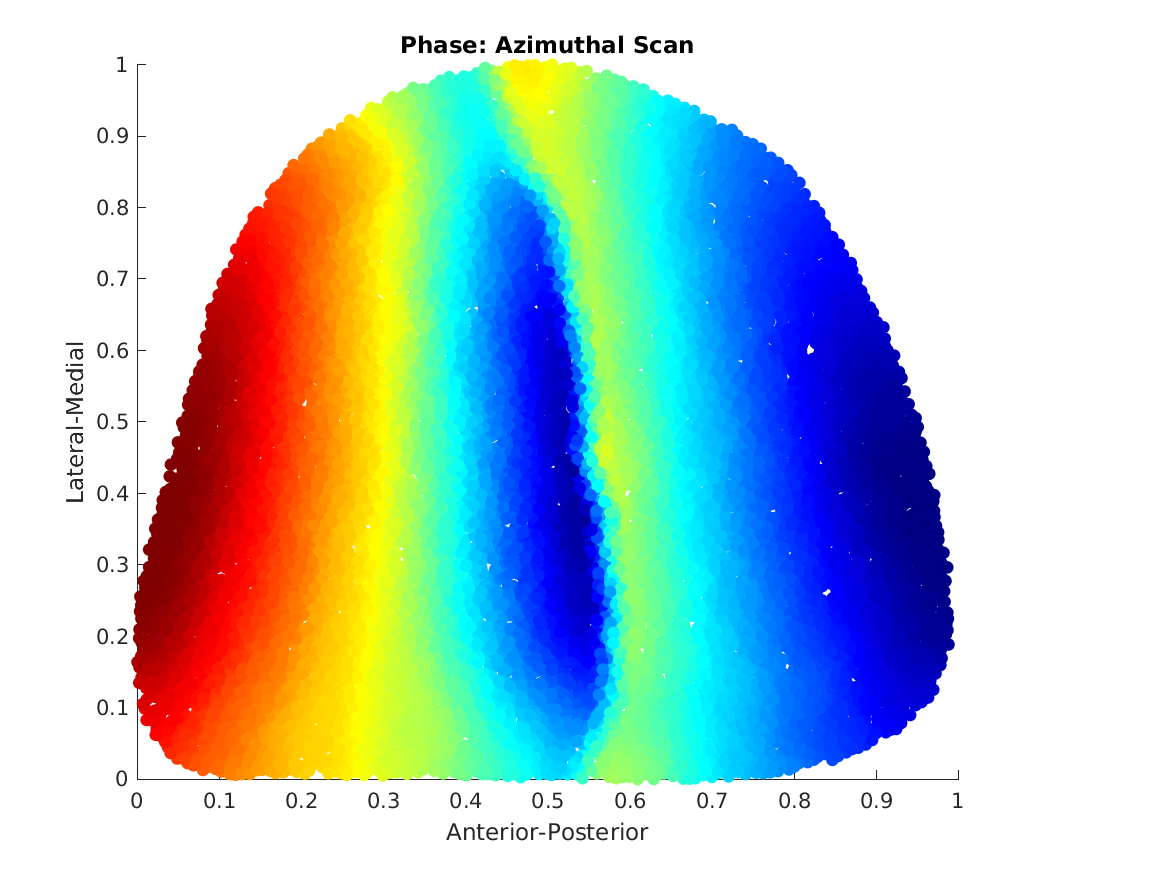
\includegraphics[width=\textwidth]{images/lattice/hetA_DR08}
		\caption{\textbf{HETA: $\Delta R =  0.226$}}
	\end{subfigure}
~
	\begin{subfigure}{0.45\textwidth}
		\centering
		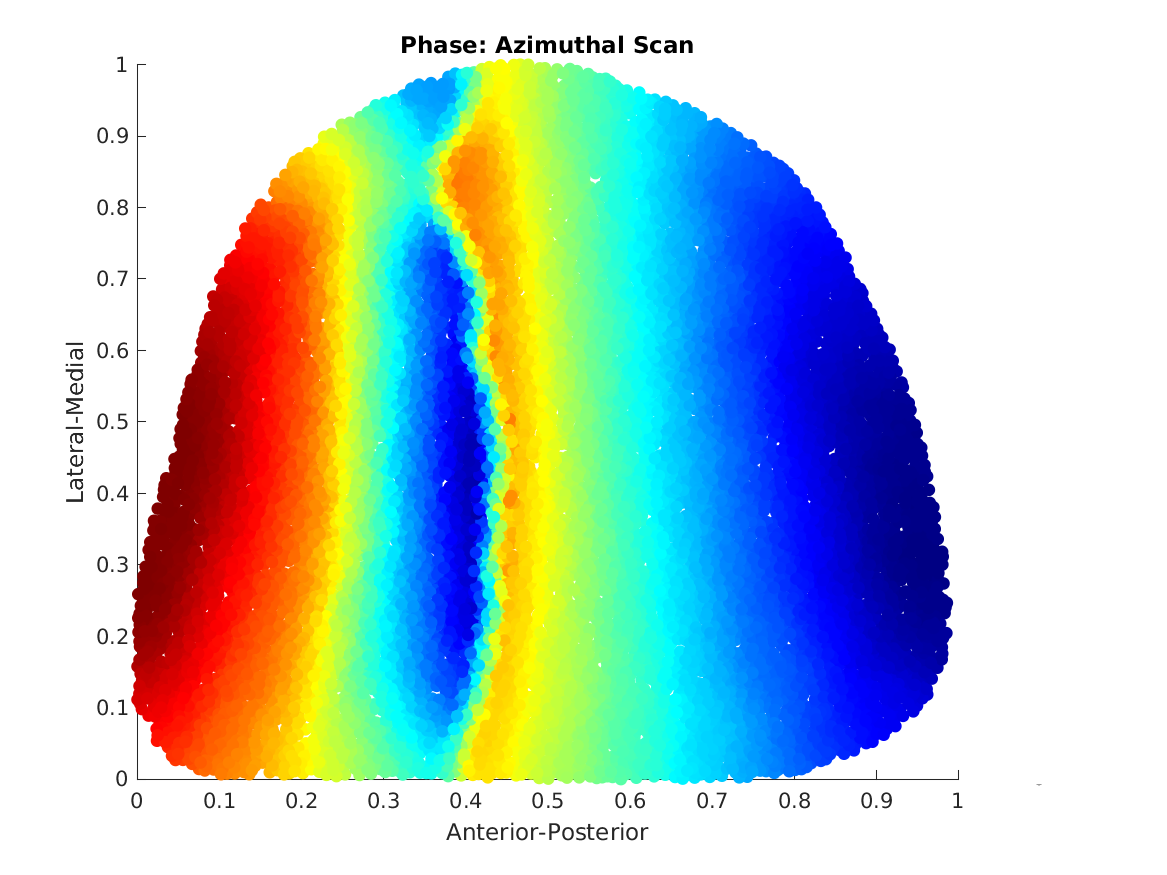
\includegraphics[width=\textwidth]{images/lattice/HetB_DR_10}
		\caption{\textbf{HETB: $\Delta R =  0.282$}}
	\end{subfigure}

	\begin{subfigure}{0.45\textwidth}
	\centering
	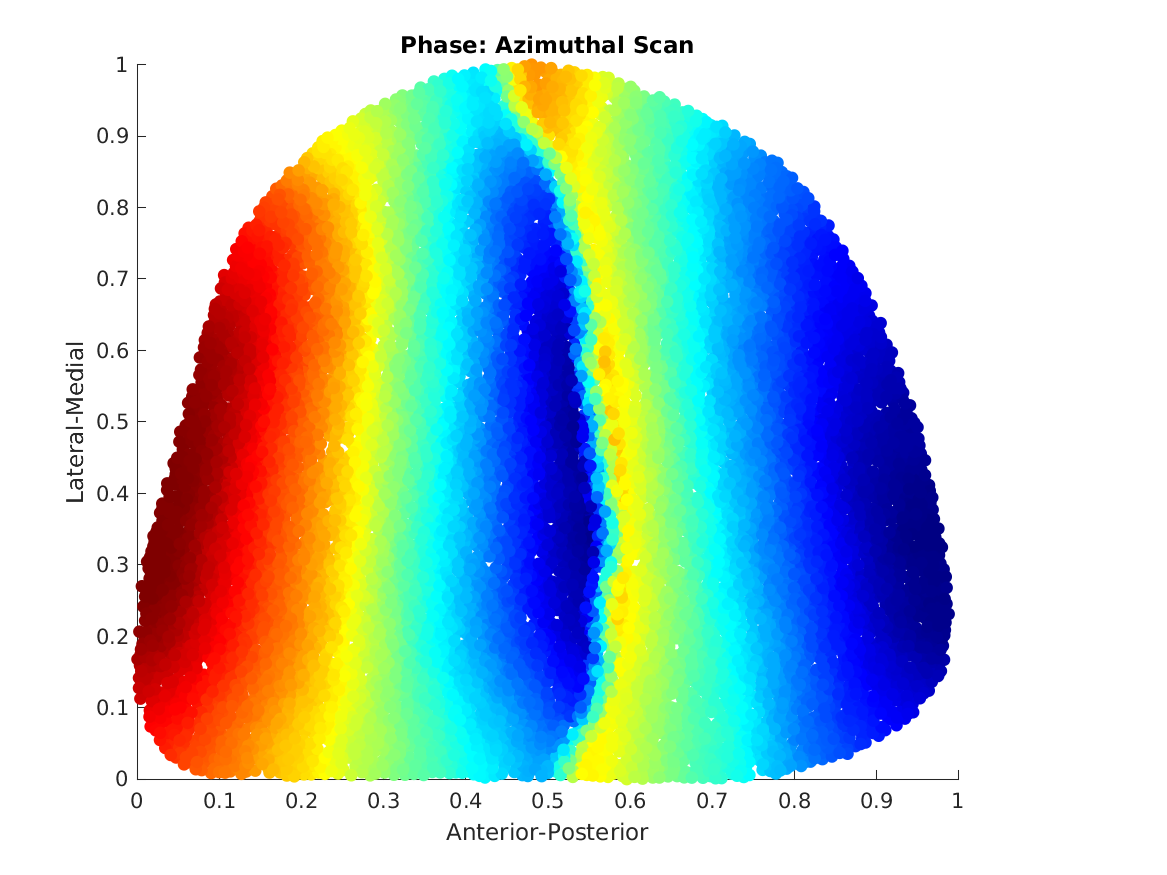
\includegraphics[width=\textwidth]{images/lattice/hetB_DR_12}
	\caption{\textbf{HETC: $\Delta R =  0.339$}}
	\end{subfigure}
~
	\begin{subfigure}{0.45\textwidth}
		\centering
		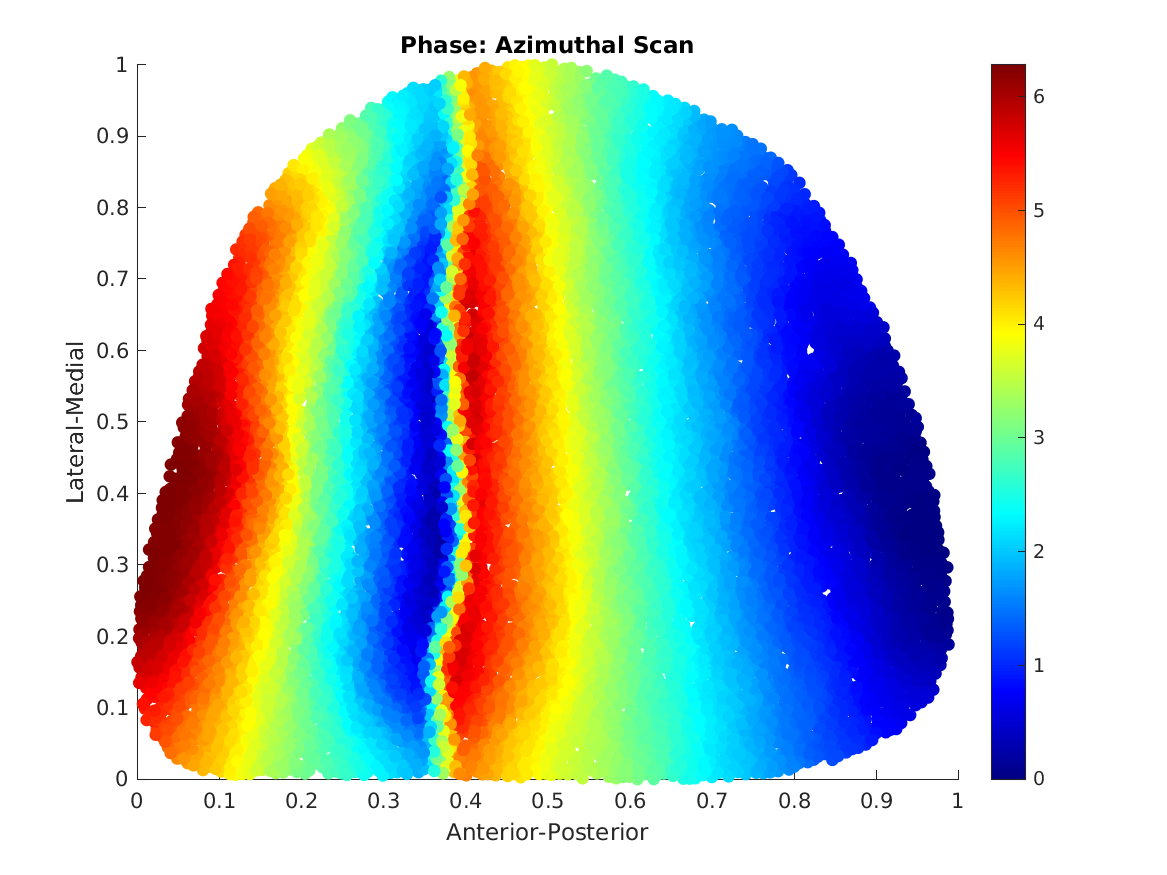
\includegraphics[width=\textwidth]{images/lattice/hom}
		\caption{\textbf{HOM: $\Delta R =  0.565$}}
	\end{subfigure}
	\def\c{The azimuthal phase diagrams for several heterozygote simulations and a homozygote simulation. }
	\caption[\c]{\c Panel (a) resembles a HETA type classification, Panel (b) resembles a HETB type classification, Panel (c) resembles a HETC type classification, and Panel (d) resembles a HOM classification. This demonstrates that under choices which correspond to experimentally observed knock-in values the optical imaging procedure can qualitatively reproduce the properties of the functional imaging data in biological specimens \cite{Reber2004-wq, Owens2015-zv}.} \label{fig:scans} 
\end{figure}
\FloatBarrier
\newpage
\paragraph{Whole Maps and Part Maps}
The differences between whole maps and part-maps are highlighted in Figure \ref{fig:wholemap}. The maps are constructed as projections from colliculus (black) and to colliculus (blue). The removed links in red when constructing the whole map are pervasive and indicate a lower quality map. By subdividing the region into two sections in the colliculus-to-field projection, or by conditioning on the cell type provenance in the field-to-colliculus projection the resulting part-map have a much higher quality. This subdivision is made automatically by finding the average rostrocaudal position of the cells that are filtered out in the data preprocessing stage; these filtered cells have a high variability in phase and likely indicate the boundary of the two populations. In the HET type simulation this provides evidence for two projections and this technique is used to analyse the effect of varying EphA3 in creating a detectable secondary projection.


\paragraph{Lattice Analysis of Varying EphA3 magnitude}
Two series of lattices, both derived from stimulating the colliculus and then using the associated phase-visual field link proposed by Kalatsky and Stryker (2003) to construct the lattice, were generated: the first selects points from the colliculus and projects into the field, the second projects from the field into the colliculus. To examine the evidence for a second projection appearing with increasing $\Delta R$ part-map lattices are constructed. These lattices are constructed in both directions and after filtering are shown in Figure \ref{fig:partmapsCTOF}. In each lattice the projection overlap is presented in purple. 
\begin{figure}
	\def\c{The colliculus-to-field part maps are shown in order of increasing $\Delta R$. }
	\caption[\c]{ Image on the following page. The colliculus-to-field part maps are shown in order of increasing $\Delta R$: the top row increases $\Delta R$ from wild-type levels up to HET levels, while the bottom row increases up to HOM levels. These levels are calibrated against the relative differences in measured mRNA expression levels for wild-type and EphA3 mice \cite{Reber2004-wq}. The noise introduced by the optical imaging procedure in the region of intermingling maps increases with $\Delta R$ mimicking biological observations. Both the rostral and caudal regions from a progressively larger cover of the visual field but the rostral region is of slightly lower quality. This is likely due to the compression of the EphA3 projection into the rostral region of the colliculus. \label{fig:partmapsCTOF}}
\end{figure}
\begin{landscape}
\begin{figure}[h!]
\hrule width1.505\textwidth
~\unskip\ \vrule\ 
\begin{subfigure}{0.475\textwidth}
	\caption{\textbf{WT: $\Delta R =  0.0$}}
	\includegraphics[width=\textwidth]{images/lattice/lattice_CTOF_0}
\end{subfigure}
~\unskip\ \vrule\ 
\begin{subfigure}{0.475\textwidth}
	\caption{\textbf{$\Delta R =  0.113$}}
	\includegraphics[width=\textwidth]{images/lattice/lattice_CTOF_04}

\end{subfigure}
~\unskip\ \vrule\ 
\begin{subfigure}{0.475\textwidth}
	\caption{\textbf{HET: $\Delta R =  0.226$}}
	\includegraphics[width=\textwidth]{images/lattice/lattice_CTOF_08}
\end{subfigure}
~\unskip\ \vrule\ 

~\unskip\ \vrule\ 
\begin{subfigure}{0.475\textwidth}
		\caption{\textbf{HET: $\Delta R =  0.339$}}
	\includegraphics[width=\textwidth]{images/lattice/lattice_CTOF_12}

\end{subfigure}
~\unskip\ \vrule\ 
\begin{subfigure}{0.475\textwidth}
		\caption{\textbf{$\Delta R =  0.452$}}
	\includegraphics[width=\textwidth]{images/lattice/lattice_CTOF_16}

\end{subfigure}
~\unskip\ \vrule\ 
\begin{subfigure}{0.475\textwidth}
		\caption{\textbf{HOM: $\Delta R =  0.565$}}
	\includegraphics[width=\textwidth]{images/lattice/lattice_CTOF_20}

\end{subfigure}
~\unskip\ \vrule\ 
\hrule width1.505\textwidth
\end{figure}

\begin{figure}[h!]
	\hrule width1.505\textwidth
	~\unskip\ \vrule\ 
	\begin{subfigure}{0.475\textwidth}
		\caption{\textbf{WT: $\Delta R =  0.0$}}
		\includegraphics[width=\textwidth]{images/lattice/lattice_FTOC_0}
	\end{subfigure}
	~\unskip\ \vrule\ 
	\begin{subfigure}{0.475\textwidth}
		\caption{\textbf{$\Delta R =  0.113$}}
		\includegraphics[width=\textwidth]{images/lattice/lattice_FTOC_04}
		
	\end{subfigure}
	~\unskip\ \vrule\ 
	\begin{subfigure}{0.475\textwidth}
		\caption{HET: $\Delta R =  0.226$}
		\includegraphics[width=\textwidth]{images/lattice/lattice_FTOC_08}
	\end{subfigure}
	~\unskip\ \vrule\ 
	
	~\unskip\ \vrule\ 
	\begin{subfigure}{0.475\textwidth}
		\caption{\textbf{HET: $\Delta R =  0.339$}}
		\includegraphics[width=\textwidth]{images/lattice/lattice_FTOC_12}
		
	\end{subfigure}
	~\unskip\ \vrule\ 
	\begin{subfigure}{0.475\textwidth}
		\caption{\textbf{$\Delta R =  0.452$}}
		\includegraphics[width=\textwidth]{images/lattice/lattice_FTOC_16}
		
	\end{subfigure}
	~\unskip\ \vrule\ 
	\begin{subfigure}{0.475\textwidth}
		\caption{\textbf{HOM: $\Delta R =  0.565$}}
		\includegraphics[width=\textwidth]{images/lattice/lattice_FTOC_20}
		
	\end{subfigure}
	~\unskip\ \vrule\ 
	\hrule width1.505\textwidth
\end{figure}
\end{landscape}

\addtocounter{figure}{-2}
\begin{figure}[h!]
	\centering
	\def\c{The field-to-colliculus part maps follow the same convention as Figure \ref{fig:partmapsCTOF} and present several notable features. }
	\caption[\c]{Image on the proceeding page. \c The distinction between the EphA3 and wild-type projections is apparent in the relative densities of the lattice map that the algorithm generates. The wild-type projection predominately inhabits the caudal region but can be seen to overlap into the far rostral region until very high levels of $\Delta R$.  \label{fig:partmapsFTOC}}
\end{figure}
\subsection{Statistical Discrimination of Phenotypes}
A generative modelling pipeline with which to query phenotypical presentations of a given genotype has been established. The principle question is whether the model supports a value for $\Delta R$ which can present as a homozygous phenotype and wild-type phenotype for different model runs. To assess this it is reasonable to ask whether there are significant differences in a sample lattice summary statistic which would reliably discriminate between a homozygote and wild-type. A useful discriminating statistic is the visual field overlap (VFO) introduced in Willshaw and Gale (2022) \cite{Willshaw2022-fs}. The VFO is computed by segregating the caudal and rostral parts of the colliculus and generating a lattice onto the visual field for both parts and recording the fraction of visual field which is represented in both maps. In the wild type there should be no overlap as the map is injective while in the homozygote the overlap should approach one. If the heterozygotes stochastically present as both of these phenotypes then a significant overlap in the distributions of the means of the EphA3$^{+/-}$ VFO with either the wild-type, homozygotes or both can be expected.
\begin{figure}[h]
	\centering
	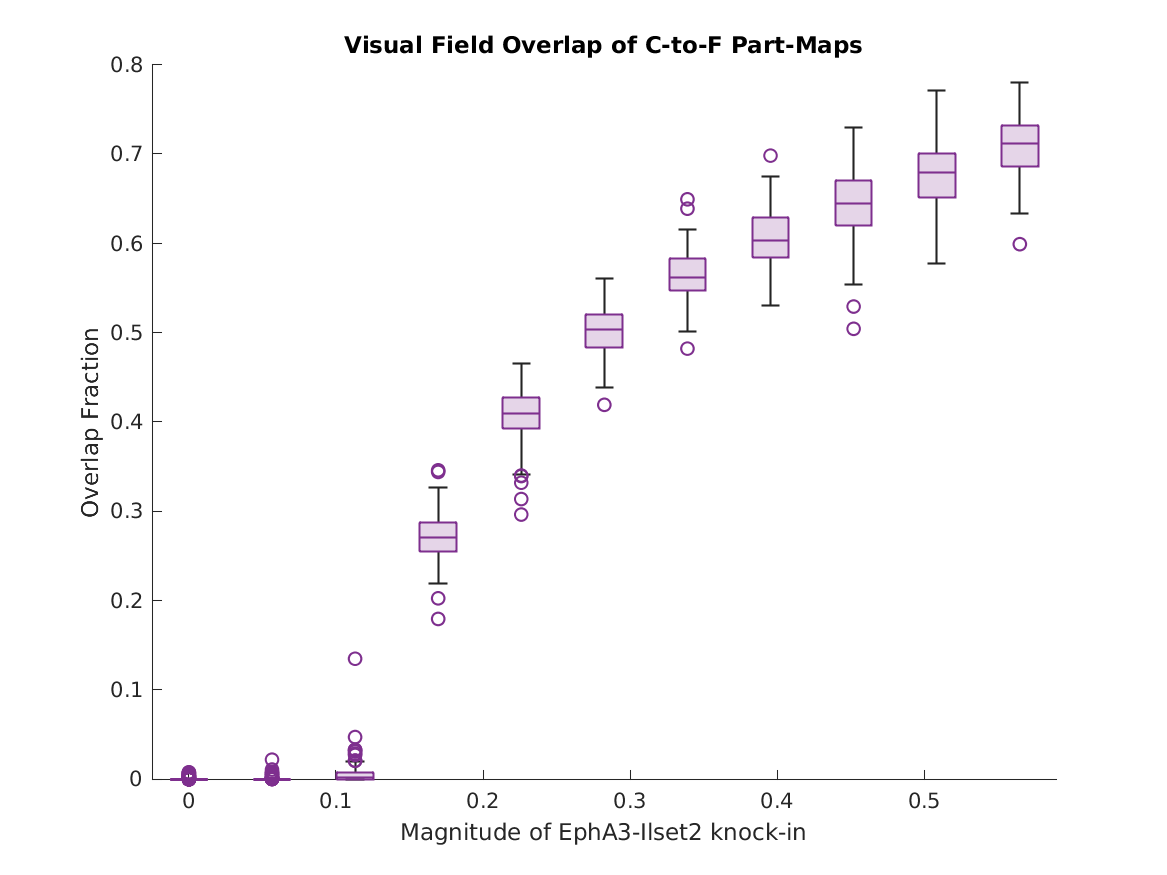
\includegraphics[width=0.75\textwidth]{images/lattice/stats_largest_vfo}
	\def\c{The VFO distributions are shown as a function of increasing EphA3. }
	\caption[\c]{\c There is a notable critical value at approximately $\Delta R=0.0565$ to $\Delta R=0.113$ where the VFO becomes no-zero. It then smoothly increases up to a value of 0.8 at the homozygous level of $\Delta R = 0.0565$. The distributions imply that at the experimentally measured levels of EphA3 knock-in for homozygotes and heterozygotes it is not likely that they can come from the same distribution. \label{fig:vfostats}} 
\end{figure}

Examining statistical hypotheses with this model is challenging due to its computationally demanding minimization procedure. A single run at the resolution of $N = 10000$ takes approximately 20 hours to converge on a single thread. The search can be distributed but even with hundreds of threads available it is prohibitively costly to examine many parameters. To alleviate the computational burden the resolution is reduced to $N = 2000$. The parameter set $\Delta R = \{0.0565 i\}_{i=0}^{i=10}$ was examined and  a modest sample of 100 maps was generated for each parameter value. This computation was distributed on 24 process using MATLABs parallel computing environment. The visual field overlap statistics are presented in Figure \ref{fig:vfostats} alongside the map quality for each of the whole and part maps, and the mean projection location of the wild-type and $Islet2$-EphA3 cells. The visual field overlap is 0 until $\Delta R = 0.113$ where it starts climbing to a maximal value of $0.9$ for $\Delta R = 0.565$. The mean projection location of the two cell types are shown in Figure \ref{fig:meanprojectionstats} where the two projections can be seen to smoothly separate for increasing $\Delta R$. The two projections have a significantly different mean at $\Delta R = 0.169$. The whole map and part-map qualities are shown in Figure \ref{fig:mapquality} where it is seen that whole map quality begins to rapidly deteriorate at $\Delta R = 0.226$ and the part map qualities initially decrease before recovering to levels of approximately 90\%. The statistics run in tandem and become significant discrimination tools at $\Delta R > 0.226$ corresponding well with the measured value of $\Delta R \approx 0.23$ \cite{Hjorth2015-le}. 

Notably, the collicular overlap does not have a dependence on $\Delta R$. Whole map quality decreases with an increasing $\Delta R$ but can be restored by subdividing the colliculus into two part maps which is in line with the data analysis. The mean projection of each of the two cell types smoothly deforms away from the other.
\begin{figure}
	\centering
	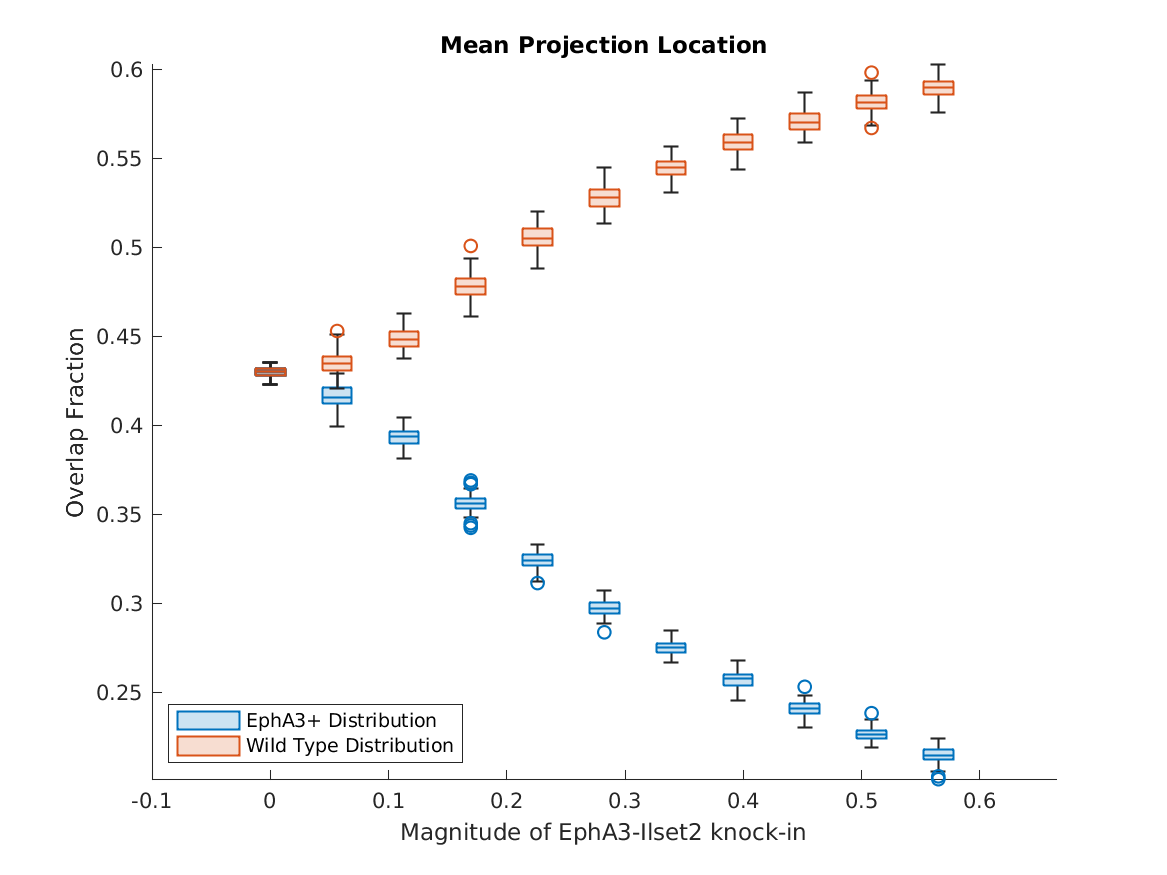
\includegraphics[width=0.75\textwidth]{images/lattice/stats_mean_projection}
	\def\c{The distributions for the mean projection location of each cell type as an increasing function of $\Delta R$.  }
	\caption[\c]{\c The projections can be seen to immediately separate and become significantly different at $\Delta R=0.169$. This validates the VFO as a measurement to discriminate the existence of two projections. \label{fig:meanprojectionstats} }
\end{figure}

\begin{figure}
	\centering
	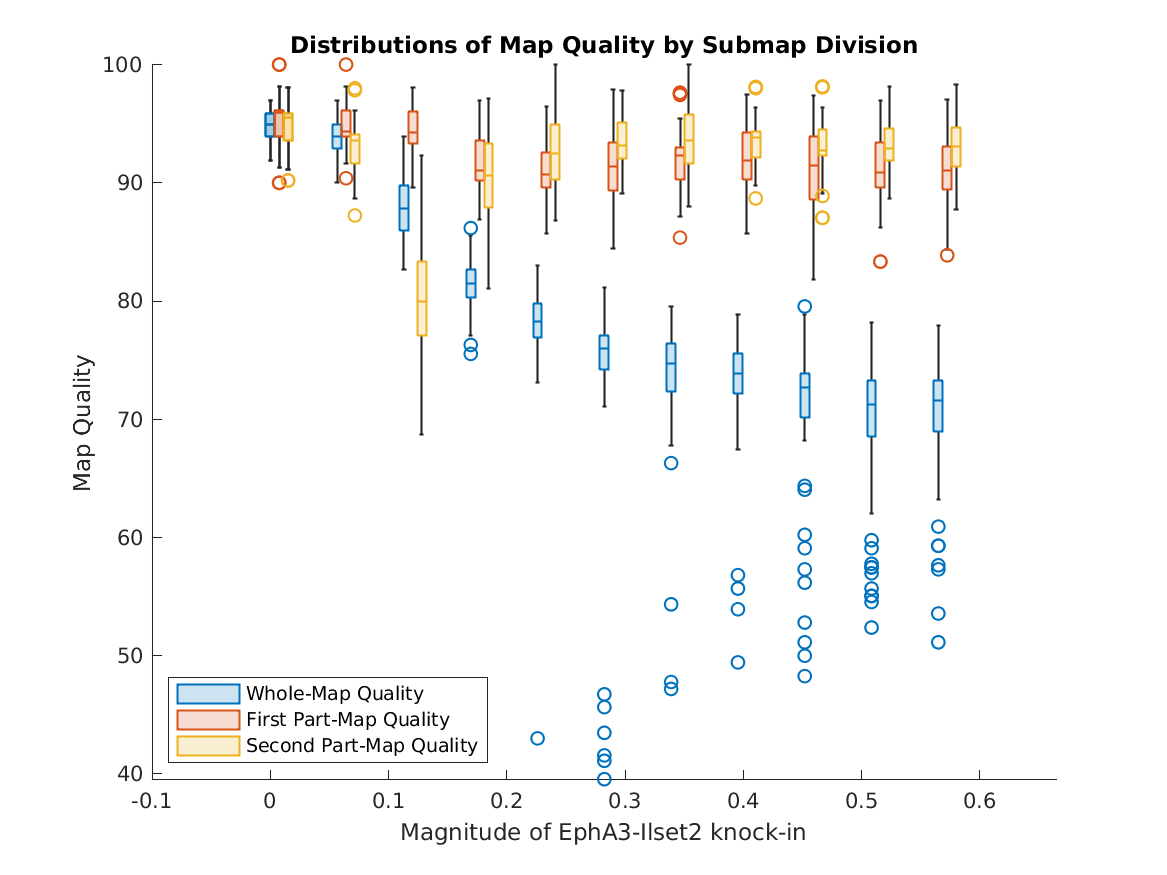
\includegraphics[width=0.75\textwidth]{images/lattice/stats_qualities}
	\def\c{Map quality distributions for the whole and individual part maps are shown in blue, red, and yellow respectively.  }
	\caption[\c]{Map quality is the percentage of nodes retained after constructing the largest ordered submap in the lattice method --- a lower quality map will have to have more nodes excluded to create a submap with topographic ordering.  \c The whole map quality begins to deteriorate at $\Delta R = 0.113$ and is significantly different from the part maps at $\Delta R = 0.226$. The whole map quality continues to decrease with increasing $\Delta R$ while the part maps remain relatively high quality for $\Delta R > 0.226$. The part-map quality returning to 90\% is quantitatively in line with the measured values for wild-type maps and part-maps biologically. This supports the existence of two distinct projections for $\Delta R > 0.226$ which corresponds well to the experimentally measured values for the additional knock-in EphA3 \cite{Hjorth2015-le}. \label{fig:mapquality} } 
\end{figure}
\FloatBarrier
\subsection{Neural Activity Perturbations}
The effects of manipulating activity on the bulk anatomical projection were examined. These were performed by manipulating the $\gamma$ parameter which scales the magnitude of the neural activity energy contribution, and $b_\text{act}$ which controls the distance over which retinal waves are correlated; see equation \ref{eq:latticemodelequation}. The first series of experiments involved increasing the $\gamma$ parameter by an order of magnitude to 0.0625 indicating a more prominent role for activity with the result of collapsing all maps into a wild-type phenotype shown in Figure \ref{fig:activitya}. The second series of experiments involved decreasing $\gamma$ by an order of magnitude to $0.000625$ which had the effect of collapsing low $\Delta R$ into a single map while reversing the polarity of the $Islet2$ expressing population shown in gold in Figure \ref{fig:activityb}. The effect of a slight increase in activity strength was examined by increasing $\gamma = 0.01$ which showed slightly tighter receptive fields but a less defined collapse point at which the two populations merged into a single map as shown in Figure \ref{fig:activityc}. A slight decrease in activity strength, shown in Figure \ref{fig:activityd}, was generated by setting $\gamma = 0.001$ and has wider receptive fields but a more defined collapse point. Finally, the activity scaling was lowered, $\gamma = 0.000625$,  and the correlation widened, $b_\text{act} = 0.2$,  mimicking the correlation results measured for the $\beta2^{-/-}$ mutant \cite{Stafford2009}. The effect of this, shown in Figure \ref{fig:activitye}, was to maintain the broad structure of the phenotypic presentation for each $\Delta R$ while widening the receptive field at each location.
\FloatBarrier
\begin{landscape}
	\begin{figure}
		\centering
		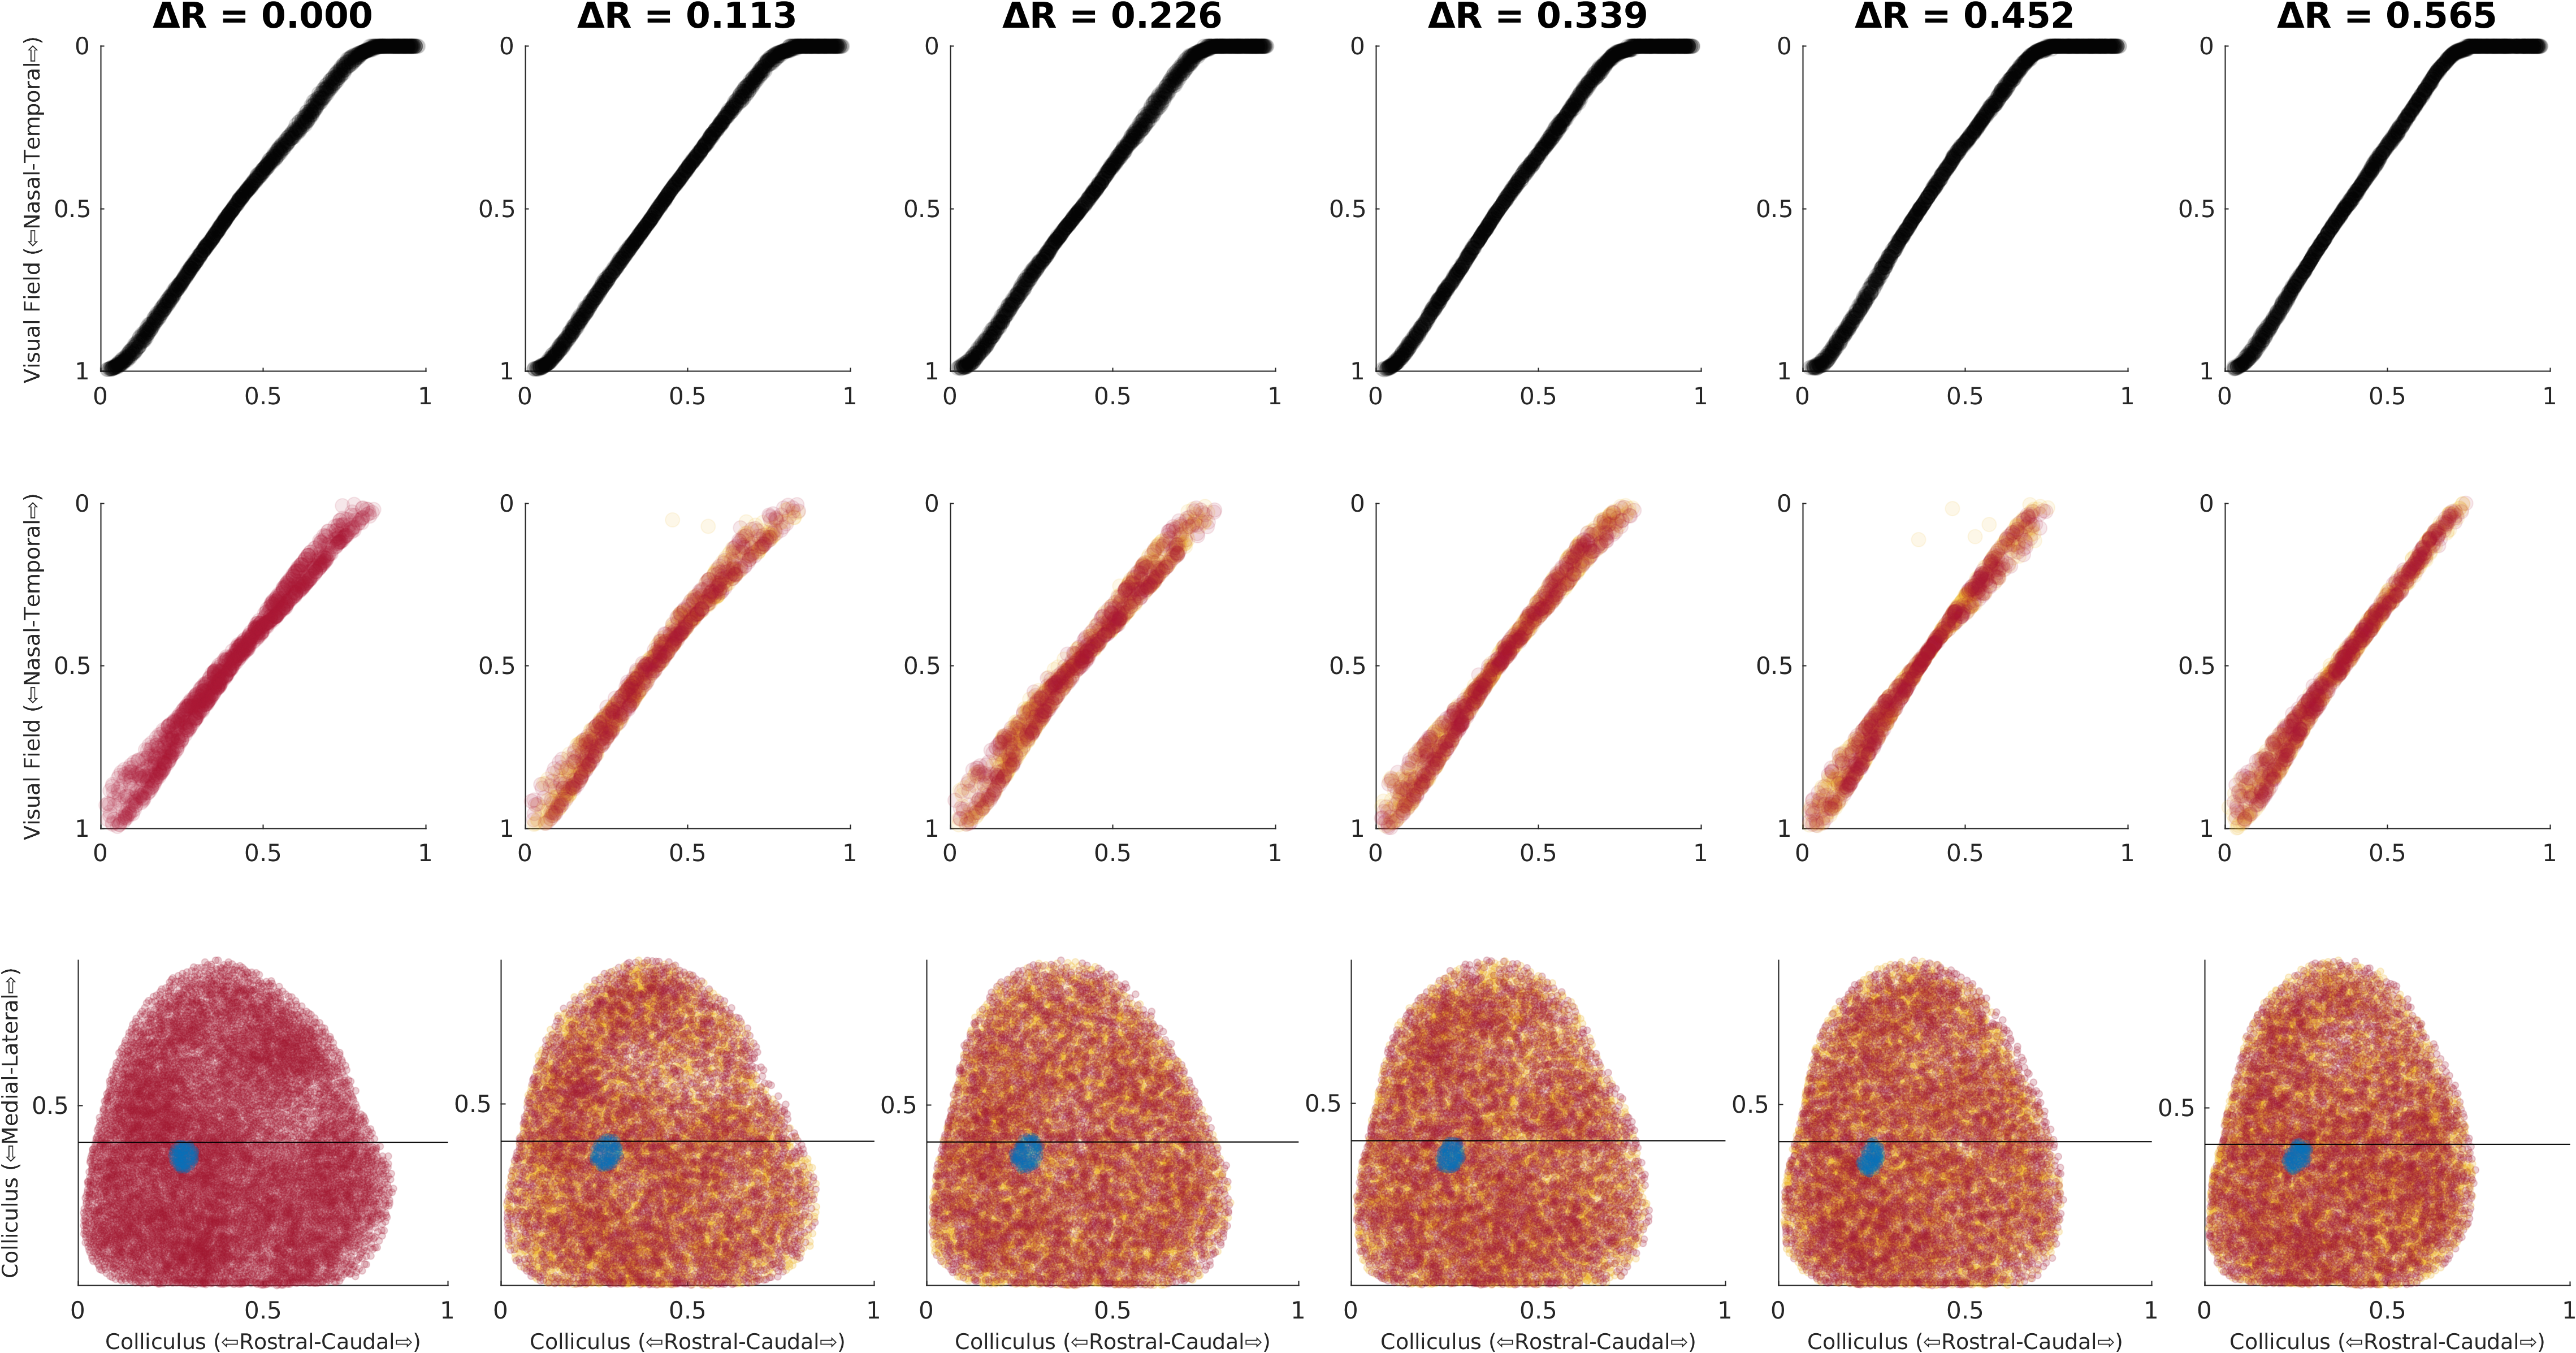
\includegraphics[width=1.6\textwidth]{images/lattice/paper_anatomy_dr_gamma_big_up}
		\captionsetup{width=.75\linewidth}
		\def\c{The activity parameter $\gamma$ is set to 0.0625 and series of injection experiments are performed on knock-in simulations with $\Delta R$ increasing left to right from $\Delta R=0$ (wild-type) to $\Delta R=0.565$ (HOM).  }
		\caption[\c]{\c This results in a complete map collapse to the wild-type phenotype across all $\Delta R$ profiles. Interestingly, the map is compressed intro the rostral colliculus for higher knock-in values. This is expected behaviour arising from the asymmetry between Eph and ephrin profiles leading to a rostrocaudal bias in the energy function. \label{fig:activitya}}
	\end{figure}
\end{landscape}

\begin{landscape}
	\begin{figure}
		\centering
		\includegraphics[width=1.6\textwidth]{images/lattice/paper_anatomy_dr_gamma_big_down}
		\captionsetup{width=.75\linewidth}
		\def\c{The activity parameter $\gamma$ is set to 0.000625 and series of injection experiments are performed as in Figure \ref{fig:activitya}. The effect of this down regulation is to introduce polarity mismatches in the EphA3 expressing cells. }
		\caption[\c]{\c These can be seen most clearly for the higher knock-in values and are characterised by a cross-hatched pattern in the centre of the map. \label{fig:activityb}}
	\end{figure}
\end{landscape}

\begin{landscape}
	\begin{figure}
		\centering
		\includegraphics[width=1.6\textwidth]{images/lattice/paper_anatomy_dr_gamma_up}
		\captionsetup{width=.75\linewidth}
		\def\c{The activity parameter $\gamma$ is set to 0.01 and series of injection experiments are performed as in Figure \ref{fig:activitya}. This slight increase in activity strength results in a less defined collapse point but slightly more refined receptive fields. }
		\caption[\c]{\c This implies that stronger activity energy contributions are enforcing a stronger notion of locality clustering points together but this introduces aberrations where there is a discontinuity at the collapse point.\label{fig:activityc}}
	\end{figure}
\end{landscape}

\begin{landscape}
	\begin{figure}
		\centering
		\includegraphics[width=1.6\textwidth]{images/lattice/paper_anatomy_dr_gamma_down}
		\captionsetup{width=.75\linewidth}
		\def\c{The activity parameter $\gamma$ is set to 0.001 and series of injection experiments are performed as in Figure \ref{fig:activitya}. This slight decrease in activity strength results in a more defined collapse point but slightly wider receptive fields. }
		\caption[\c]{\c These effects are the direct counterpart to those in Figure \ref{fig:activityc}. They arise from the lower activity energy contributions relaxing local clustering. \label{fig:activityd}}
	\end{figure}
\end{landscape}

\begin{landscape}
	\begin{figure}
		\centering
		\includegraphics[width=1.6\textwidth]{images/lattice/paper_anatomy_dr_beta2}
		\captionsetup{width=.75\linewidth}
		\def\c{The activity profile is constructed to mimic the $\beta2^{-/-}$ genotype with a wider neural activity correlation profile and series of injection experiments are performed as in Figure \ref{fig:activitya}. }
		\caption[\c]{\c The effects are most similar to those shown in Figure \ref{fig:activityd} but they arise for different reasons. The receptive fields are broadened because of the decreased gradient of the activity energy resulting in similarities in energy between cells at a greater distances. These similarities make it difficult to discriminate a local boundary as opposed to a removal of the effect of activity energy contributions and effects.  \label{fig:activitye}}
	\end{figure}
\end{landscape}

\section{Discussion}
The data presented here gives qualitative and quantitative measures by which to benchmark the model analyses. In the data reanalysis reviewed here the variability observed by Owens et. al. (2015) has been broken into subclasses which have validated their observations (Willshaw and Gale, 2022) \cite{Willshaw2022-fs}. The model is able to reproduce optical imaging experiments and maps qualitatively as well as key phenomenological features. The model reproduces faithful representations of magnification effects. Assuming the means are distributed normally then the distributions generated by the model are most similar to the HET classes of data in the range $0.113-0.169$ under both the map quality and VFO statistics. The HOM class is more challenging to interpret with map quality being most similar to the distributions in the upper limits of the $\Delta R$ range but with VFO being most similar in the range $0.169-0.226$. This challenges the observations of the phase maps which give the best qualitative matches in the range $0.226-0.339$ for the heterozygotes and $0.508-0.565$ for the homozygotes and these values are more consistent with  previous modelling estimates. The mismatch between the level predict qualitatively by visual inspection of the phase map and quantitatively by measured statistics warrants further investigation. There are two principle areas of concern: data number and model resolution. The number of specimens examined were very low, $<$5 for the HOM class, and it is unlikely that this formed a representative sample. The model resolution used to generate the theoretical distribution was reduced by a factor of 5 for reasons of computational efficiency and this low resolution may mar the predicted distributions; there are notably more outliers for higher $\Delta R$. To summarise, the model provides an adequate representation of the biological data conditioned on the low sample number and discussion is turned to theoretical implications.
\paragraph{Proportion of EphA3 Cells}
For each of the $\Delta R$ experiments proportion of EphA3 cells was varied between 40\%, 50\% and 60\%. These experiments do not affect the principle results and have been omitted for this chapter but may be found at \cite{LatticeEphA3}. In brief, the effect of increasing the number of EphA3 cells is to increase the area of the superior colliculus which they occupy (Willshaw and Gale, 2022) \cite{Willshaw2022-fs}. 
\paragraph{Neural Activity Modelling}
Modelling the effect of the $\beta2^{-/-}$ perturbations to activity is non-trivial. Recent studies suggest that in the Tsigankov-Koulakov model the chemical cues must be scaled in tandem with the activity cues \cite{Lyngholm2019-fs}. For this reason the primary focus has been modelling the $\beta2^{-/-}$ expressing variant for which the Tsigankov-Koulakov model has been validated, and indeed designed for. Several pilot studies modifying the scale of activity ($\gamma$) but not the correlation width were conducted and the results suggest that regular retinotopy can be recovered if the activity is completely dominant ($\gamma = 0.0625$) but lowering the activity by an order of magnitude $(\gamma = 0.00625)$ results in a collapse into wild-type phenotypes for low $\Delta R$ in support of the principle hypothesis but maps with disordered polarity for high $\Delta R$; see Figure \ref{fig:activitya} and \ref{fig:activityb}. When the activity scaling is perturbed marginally upward $(\gamma = 0.01)$ the phenotypes maintain similar structure to normal activity levels but with a less pronounced mapping collapse and marginally tighter receptive fields, while when the activity was slightly lowered ($\gamma = 0.001)$ this mapping collapse became more pronounced which could be due to a dominance of the chemotactic mechanism \cite{Willshaw2022-fs}.  When the activity strength was lowered and the correlation window was widened the polarity effect disappeared and the map phenotypes remained the same profile as those with normal activity patterns but with widened receptive fields; see Figure \ref{fig:activitye}. This is consistent with the general hypothesis that chemotaxis establishes broad topographic patterns and neural activity refines these with the $\beta2^{-/-}$ knock-out have less refining capability.

Due to a lack of available data and small number of mutants tested by Owens et. al. (2015) this could not be rigorously tested but in the context of the reported effects this suggests that the activity strength is significantly increased in the $\beta2^{-/-}$ knock-out which is would be a departure from the consensus in the literature \cite{Owens2015-zv, Stafford2009}.  The lattice plots for these experiments have not been included as they are consistent with the interpretations drawn from the anatomy. A potential explanation for the observation of wild-type phenotypes in EphA3$^{+/-}\beta2^{-/-}$ mice is that the retinal arbours are simply not refined enough to be phase differentiated. The optical imaging process involves a convolution over the projection of each retinal afferent and injection experiments show that in $\beta2^{-/-}$ this projection is a significant portion of the colliculus \cite{McLaughlin2003-yy, Burbridge2014-ib}. This means the phases will be averaged out over large areas and will only distinguish slight biases between each boundary. This hypothesis is consistent with visual inspection of the data but due to a lack of quantitative data this was not tested rigorously. It is clear that the activity-chemotaxis interplay alters map formation but modelling cannot reconcile nor reproduce the effect shown by Owens et. al. (2015) in the context of the current parameter space and with available activity profiles \cite{Owens2015-zv}.  
\paragraph{Anatomical Segregation}
Te anatomical region which each EphA3 cell is bound is seen to be a smooth function of $\Delta R$; see Figures \ref{fig:antomicalEphA3} and \ref{fig:partmapsFTOC}. The wild-type cells have a more complicated relationship and appear to consistently attempt to project over the whole colliculus and are slowly removed from the EphA3 domain with increasing $\Delta R$. At high $\Delta R = 0.565$ the populations are nearly completely segregated implying the two functional domains observed have been formed of two analogously cell differentiated anatomical maps \cite{Cang2013-dw}. However, the EphA gradient is normalised to take a maximal value of 1 and data reported from mRNA expression suggests that the additional EphA contributes approximately 0.525 of the maximal value in homozygotes and 0.243 in heterozygotes \cite{Reber2004-wq}. At these levels the model does not predict a a complete anatomical segregation of the two populations but rather a well defined and constrained EphA3 map restricted to the caudal region and a wild-type map which covers the whole colliculus but has significantly lower coverage in the in the EphA3 dominated region. Through this parameter sweep the EphA3 dominated region is well conserved and smoothly deforms to the final segregated state which is evidence that the maps are not stochasticly organising individual domains but rather that aberrations in the phase map are derived from phase analysis artefacts from interacting signals with differing retinal provenance.
\paragraph{Lattice Analysis}
The Lattice method gives topological insight into how the EphA3 projection is deformed from wild-type to homozygote with increasing $\Delta R$. The lattice plots show that this deformation happens smoothly with two maps being developed on top of each other. The maps slowly segregate and as they do they compete less with each other and develop strong complete representations of the visual field. 

The two representations can be identified and classified as rostral or caudal on the basis of activity variability under stimulation. This correlates well with the observed data used to construct the maps and can be used to make a direct comparison. A measure of the deformation can be found by computing the VFO statistics on both the model comparing it with the VFO computation for the data. In the model the deformation is relatively smooth with increasing $\Delta R$; see Figure \ref{fig:vfostats}.
\paragraph{Variability in the EphA3 knock-in}
The above considerations allow for commentary on the variability and anatomy of the EphA3 mutant both in the heterozygote and homozygote case. In the heterozygote case the data shows a large degree of variability in the optical imaging scans which the model can reproduce qualitatively. The source of this variability is unlikely to be the anatomy as the results show the two anatomical projections are reasonably smoothly deformed and well constrained in the colliculus. If the variability were to come from the amount of EphA3 present in the $Islet2$ expressing cells then there would be a large range of potential EphA3 inserted stochastically between each individual specimen. This would lead to significant VFO overlap between HET, HOM, and wild-type classifications which have not been observed. This seems unlikely in the context of the measured EphA3 knock-in levels but warrants further investigation \cite{Reber2004-wq}. This leaves the variability in the signal. Given the noise present in the data and the requirement to filter out large portions of colliculus it would appear that the overlapping anatomical projections and stochastic processes involved with the signal generation interact to generate the phase aberrations seen in the data. There will of course be anatomical variations which lead to different signal interactions but the developmental process does not appear to be largely stochastic and is instead reasonably well ordered.

This argument also allows for commentary on the likely anatomy of the EphA3 homozygote which has been argued to completely segregate in the colliculus \cite{Cang2013-dw}. The whole field injections demonstrate that for complete segregation of the $Islet2$-EphA3 and wild-type cells the EphA3 knock-in must be more than double the maximal value of the regular EphA gradient. This seems unlikely given the measured EphA3 knock-in value derived from mRNA expression levels \cite{Reber2004-wq}. The optical imaging pipeline suggests that anatomical segregation is not a requirement for an measured functional duplication; see Figure \ref{fig:scans}. If the $Islet2$ positive and negative cells can be differentially colour tagged with fluorescent proteins the model predicts a flood injection would reveal wild-type projections in the caudal region occupied predominately by EphA3 type cells. This is an experimentally falsifiable hypothesis.
\paragraph{Limitations}
There are several theoretical and biological limitations in this study: large computational cost, an inconclusive understanding of the interaction of the model mechanisms, and an inability to reproduce the $\beta2^{-/-}$. The computational cost of the model is the most severe --- a single execution currently takes an entire day. This cost severely hampers statistical methods, such as MCMC, to be applied to data and requires parameters to be tuned by hand. This parameter tuning has resulted in several generations of model parameters which limit interpretability; see Section \ref{sec:efficientmodelling}. In this study a basic understanding of the distributions generated by the model were obtained by using a much lower resolution: 2000 cells versus the 10000 cells used to complete the displayed lattice plots and anatomical tracing studies. Perhaps as a result of this limitation the relative interaction between model mechanisms is not well understood; a study of the developmental time course of the $\beta2^{-/-}$ mutant was able to recover biological plausibility by unintuitively scaling the chemotactic parameters, not activity \cite{Lyngholm2019-fs}. This study performed some basic pilot studies of activity manipulation which corroborate the idea that neural activity acts to refine the projection; see Section \ref{section:developmentaltheory}. An extensive understanding of the interaction with the chemotactic EphA3 manipulation and activity was not developed. As a result the study was unable to reproduce the limited data presented by Owens et. al. (2015) \cite{Owens2015-zv}. The dataset was sparse (N = 2 mice) and developing both an extensive dataset and a rigorous theoretical understanding of the interaction between these two mechanisms is a good target for future theoretical work.
\paragraph{Future Work}
A basic parameter search helped gain an understanding of the statistical properties of EphA3 knock-in perturbations in this work. This was achieved by access to a high-performance computing cluster and simultaneously it was necessary to reduce the resolution of the model thereby reducing its explanatory power. These limitations were imposed by the computationally demanding minimisation procedure employed by the model. In addition, the model parameters were tuned by hand which is useful for exploration but is not scientifically desirable. Furthermore, the parameters in the neural spiking model used to replicate the intrinsic optical imaging procedure were selected as a first order approximation of existing biological data \cite{Phongphanphanee2014-in}. A more rigorous approach would be defining the parameters via Bayesian regression on the available data which would allow current prior beliefs to be encoded; such an analysis was performed in Chapter \ref{chapter:neuralstdp}. This approach is entirely unfeasible even with massive parallelisation: the wall time of a single run at high resolution is approximately 20 hours and thousands of runs would be needed for an MCMC to converge \cite{Gelman1995-uj}. This procedure would allow the data to dictate the relative strength of activity and chemotaxis which is not currently biologically measurable and this relative strength would more rigorously guide theoretical investigations of the interactions between these two mechanisms. It is therefore desirable to design a framework which is computationally efficient enough to be amenable to rigorous parameter and data analysis while maintaining the phenomenological account of the various genotypes. A procedure for assessing the second criteria was given by Hjorth et. al. (2015) \cite{Hjorth2015-le}. The principles embodied in existing models and outlined in Section \ref{sec:models} will be used in the next chapter to develop a modelling framework that is computationally efficient.
\paragraph{Key Summary}
\begin{enumerate}
	\item \textit{An extensive theoretical examination of the EphA3 mutant was performed to further explore the data presented by Owens et. al. (2015) and to corroborate and understand the data analysis performed by David Willshaw  \cite{Willshaw2022-fs, Owens2015-zv}.}
	\item \textit{The analysis used the Tsigankov-Koulakov model to generate an underlying anatomical representation of the retinotopic projection and then used this in conjunction with a neural spiking model to generate an intrinsic optical imaging scan and thus replicating the entire experimental pipeline \cite{Kalatsky2003-cz, Owens2015-zv}.}
	\item \textit{Lattice analysis and anatomical tracer injections were performed revealing the model adequately explains experimental observations. A parameter sweep of the amount of EphA3 revealed that there is not likely to be a stochastic activity-chemotactic component to the development of EphA3 mutants but rather a smooth deformation with the increase in EphA3}.
	\item \textit{A moderate amount of samples of a low-resolution implementation of the model were generated and used to compute statistics generate by the lattice method. The VFO and mean projection location of the two cell types demonstrate the smooth transition while presenting evidence that heterozygotes are unlikely to present as homozygotes and wild-type.}
	\item \textit{The model predicts that even for high (homozygote) levels of EphA3 knock-in there is intermingling between the $Islet2^{+/-}$ and $Islet2^{-/-}$ cells. Previous work suggested, these populations completely segregate in the colliculus and this presents a falsifiable hypothesis \cite{Cang2013-dw}.}
\end{enumerate}